\documentclass[twoside,11pt]{article}

% Any additional packages needed should be included after jmlr2e.
% Note that jmlr2e.sty includes epsfig, amssymb, natbib and graphicx,
% and defines many common macros, such as 'proof' and 'example'.
%
% It also sets the bibliographystyle to plainnat; for more information on
% natbib citation styles, see the natbib documentation, a copy of which
% is archived at http://www.jmlr.org/format/natbib.pdf

\usepackage{jmlr2e}

% package we use can go here
\usepackage{comment}
\usepackage{amsmath}
\usepackage{amssymb}
\usepackage{amsfonts}
\usepackage{url}
\usepackage{natbib}
\usepackage{epsfig}
%\usepackage{subfigure}
\usepackage{subfig}
\usepackage{graphicx}
\usepackage{xcolor}
\usepackage{multirow}
\usepackage{paralist}
\usepackage[ruled]{algorithm2e}
\SetKwRepeat{Do}{do}{while}

% Definitions of handy macros can go here
%%%%%% vectors
\def\b0{{\bf 0}}
\def\ba{{\bf a}}
\def\bb{{\bf b}}
\def\bd{{\bf d}}
\def\be{{\bf e}}
\def\bi{{\bf i}}
\def\bh{{\bf h}}
\def\bm{{\bf m}}
\def\br{{\bf r}}
\def\bs{{\bf s}}
\def\bu{{\bf u}}
\def\bv{{\bf v}}
\def\bw{{\bf w}}
\def\bx{{\bf x}}
\def\by{{\bf y}}

%%%%%% sets
\def\real{{\mathbb{R}}}
\def\R{\mathbb{R}}
\def\Obs{\Omega_{obs}}
\def\dist{{\mathcal D}}

%%%%%% operators and functions
\newcommand\Ex[2]{{\mathbb E}_{#1}\big[#2\big]}
\newcommand\btrace[1]{{\operatorname{trace}}\left(#1\right)} % big trace
\newcommand\bsign[1]{\operatorname{sign}\left(#1\right)} % big () for sign function
\newcommand\trace[1]{{\operatorname{trace}}(#1)}
\newcommand\rank[1]{{\operatorname{rank}}(#1)}
\newcommand\sign[1]{\operatorname{sign}(#1)} % sign function
\newcommand\sgn[1]{{\operatorname{sign}}(#1)}  % sign function
\newcommand\diag[1]{\operatorname{diag}({#1})}
\newcommand\proj[1]{{\mathcal P}_{#1}}
\newcommand\inv[1]{{#1}^{-1}}
\newcommand\trans[1]{{\mathcal T}_{#1}}
\newcommand\IP[2]{\langle{#1}, {#2}\rangle}
\newcommand\sqinv[1]{{#1}^{-2}}
\newcommand\ind[1]{\mathbf{1}\left[ #1 \right]} % indicator function

\def\T{{\mathcal T}}  % thresholding operator in dirtyIMC

%%%%%% space of matrices
\def\col{\text{col}}

%%%%%% constraint parameters of optimization
\def\amax{{\mathcal A}}
\def\bmax{{\mathcal B}}
\def\mmax{{\mathcal M}}
\def\nmax{{\mathcal N}}
%\def\rmax{{\mathcal R}}
%\def\tmax{{\mathcal T}}
\def\smax{{\mathcal S}}
\def\wmax{{\mathcal W}}
\def\xmax{{\mathcal X}}
\def\ymax{{\mathcal Y}}

\def\wM{\hat{M}}
\def\wN{\hat{N}}
\def\rad{{\mathfrak R}}
\newcommand\polylog[1]{\operatorname{polylog}{#1}}

\def\gau{{\mathcal N}}
\def\DU{\Delta U}
\def\DV{\Delta V}

%%%%%% Robust PCA solutions and certificates
\def\realL{L_0}
\def\realM{M_0}
\def\realS{S_0}
\def\optL{L^*}
\def\optM{M^*}
\def\optN{N^*}
\def\optS{S^*}
\def\HL{H^L}
\def\HS{H^S}
\def\WL{W^L}
\def\WS{W^S}
\def\Kone{K^{(1)}}
\def\Ktwo{K^{(2)}}

%%%%%% operator of matrices
\def\Iop{{\mathcal I}}
\def\Rop{{\mathcal R}}
\def\Sop{{\mathcal S}}

% Heading arguments are {volume}{year}{pages}{submitted}{published}{author-full-names}

\usepackage{lastpage}
\jmlrheading{19}{2018}{1-\pageref{LastPage}}{03/17; Revised 05/18}{12/18}{17-112}{Kai-Yang Chiang and Cho-Jui Hsieh and Inderjit S. Dhillon}

% Short headings should be running head and authors last names

\ShortHeadings{Low-Rank Matrix Learning with Side Information}{Chiang, Hsieh and Dhillon}
%\ShortHeadings{Learning Low-Rank Matrices from Missing and Corrupted Entries with Side Information}{Chiang, Hsieh and Dhillon}
\firstpageno{1}

\begin{document}
\sloppy

\title{Using Side Information to Reliably Learn Low-Rank Matrices from Missing and Corrupted Observations}
\author{\name Kai-Yang Chiang \email kychiang@cs.utexas.edu\\
  \name Inderjit S. Dhillon \email inderjit@cs.utexas.edu\\
  \addr Department of Computer Science\\
  University of Texas at Austin\\
  Austin, TX 78701, USA \\
  \name Cho-Jui Hsieh \email chohsieh@ucdavis.edu\\
  \addr Department of Statistics and Computer Science\\
  University of California at Davis\\
  Davis, CA 95616, USA
}

\editor{Sanjiv Kumar}

\maketitle

\begin{abstract}%   <- trailing '%' for backward compatibility of .sty file
Learning a low-rank matrix from missing and corrupted observations is a fundamental problem
in many machine learning applications.
However,
the role of {\it side information} in low-rank matrix learning has received little attention,
and most
current approaches are either ad-hoc or only applicable in certain restrictive cases.
In this paper, we propose a general model that exploits side information to
better learn low-rank matrices from missing and corrupted observations,
and show that the proposed model can be further applied to several popular scenarios
such as matrix completion and robust PCA.
Furthermore, we study the effect of side information on sample complexity
and show that by using our model,
the efficiency for learning can be improved given sufficiently
informative side information.
This result thus provides theoretical insight into the usefulness of side information
in our model.
Finally, we conduct comprehensive experiments in three real-world applications---relationship
prediction, semi-supervised clustering and noisy image classification, showing that
our proposed model is able to properly exploit side information for more effective
learning both in theory and practice.
\end{abstract}

\begin{keywords}
  Side information, low-rank matrix learning, learning from missing and corrupted observations, matrix completion, robust PCA
\end{keywords}

\section{Introduction}
\label{sec:intro}
Learning a low-rank matrix from noisy, high-dimensional complex data is an
important research challenge in modern machine learning.
In particular, in the recent big data era, assuming that the observations come
from a model with implicit low-rank structure
is one of the most prevailing approaches to avoid the curse of dimensionality.
%and such a low-rank structure of the model has also been shown to appear in many
%real-world applications such as recommender systems~\citep{Koren09a}, video
%processing~\citep{PH96a},
%bioinformatics~\citep{OA00a} and social network analysis~\citep{Hsieh12a}.
While various low-rank matrix learning problems arise from different contexts and domains,
the primary challenge is rather similar: namely to
reliably learn a low-rank matrix $\realL$
based only on missing and corrupted observations from $\realL$.
This generic framework includes many well-known machine learning problems such as
matrix completion~\citep{Candes09a},
robust PCA~\citep{Wright09a} and matrix sensing~\citep{Zhong15a}, and is shown to be
useful in many important real-world applications including
recommender systems~\citep{Koren09a}, social network analysis~\citep{Hsieh12a}
and image processing~\citep{Wright09a}.

Among research related to low-rank matrix learning,
one promising direction %to improve the learning process
is to further exploit {\it side information}, or {\it features},
to help the learning process.~\footnote{We will use terms `side information' and `features'
interchangeably throughout the paper.}
The notion of side information appears naturally in many applications.
For example, in the famous Netflix problem where the goal is movie
recommendation based on users' ratings, a popular
approach is to assume that the given user-movie rating pairs are sampled from a
low-rank matrix~\citep{Koren09a}.  However,
besides rating history, profiles of users and/or genres of movies may also be provided,
and one can possibly leverage such side information for better recommendation.
Since such additional features
%some might be informative while others might be noisy,
are available in many applications,
designing a model to better incorporate features into low-rank matrix learning problems
%and how much features could benefit general matrix completion task,
becomes an important issue with both theoretical and practical interests.

Motivated by the above realization, %in this paper,
we study the effect of side information on learning low-rank matrices from missing
and corrupted observations in this paper.
%We start with exploiting side information for two prominent instances---matrix completion and
%robust PCA problem---where the learning is conducted under partial and corrupted observations
%respectively.
%These examples provide abundant insights on the methodology of incorporating
%side information under different circumstances,
%motivating us to further develop a unified framework for general low-rank matrix learning
%with side information.
Our general problem setting can be formally described as follows.
Let $\realL \in \R^{n_1\times n_2}$ be the low-rank modeling matrix,
yet due to various reasons we can only observe a matrix $R\in\R^{n_1\times n_2}$ which
contains missing and/or corrupted observations of $\realL$.
In addition, suppose we are also given additional feature matrices
$X \in \R^{n_1 \times d_1}$ and/or $Y \in \R^{n_2 \times d_2}$ %, $d_1, d_2 \leq n_1, n_2$
as side information,
where each row $\bx_i \in \R^{d_1}$ (or $\by_i \in \R^{d_2}$) denotes a feature representation of the $i$-th
row (or column) entity of $X$ (or $Y$).
Then, instead of just using $R$ to recover $\realL$,
our hope is to leverage side information $X$ and $Y$ to learn $\realL$
more effectively.  Below, we further list some important applications where
the side information naturally comes in as the form of $X$ and/or $Y$ in this framework:
\begin{itemize}
  \item {\it Collaborative filtering}.  Collaborative filtering is one of the most popular
    machine learning applications in industry where we aim to predict the preferences
    of users to any products based on limited rating history (e.g. the Netflix problem we
    mentioned previously).
    A traditional approach is to complete the partial
    user-product rating matrix $R$ via matrix completion.  However, one could also
    collect per-user features $x_i$ and per-product features $y_j$ as possible information
    to leverage, and the assembled
    feature representation for users and products becomes $X$ and $Y$ in this framework.
  \item {\it Link prediction}.  The link prediction problem in online social network analysis
    is to predict and recommend the implicit friendships of users given the current network
    snapshot.  One approach is to think of the network snapshot as a user-to-user relationship
    matrix $R$, and thus any missing relationships in the snapshot can be inferred by
    conducting matrix completion on $R$~\citep{Nowell07a}.
    Similarly, if user-specific
    information (like user profile) is collected, these user features can be
    deemed as both $X$ and $Y$.
  \item {\it Image denoising}.  Another low-rank matrix learning application is image
    denoising.  It is known that same types of images (e.g. images of human face, digits, or
    images with same scene) often share a common low-rank structure, and learning that
    low-dimensional space can be useful for many applications such as image recognition
    and background subtraction.  Yet
    in the realistic setting, images may be corrupted by sparse noise
    such as shadowing or brightness saturation, making the learning of that low-dimensional
    space much more difficult.  A popular approach, known as robust PCA, is
    to construct an observed matrix $R$ where each column is a vector
    representation of an image, and further learn the
    underlying low-rank subspace by separating it from the sparse noise in $R$.
    In Section~\ref{sec:exp}, we will show that if features of clean images $X$ and/or
    label-relevant features $Y$ are also given, one can learn the underlying
    low-dimensional subspace more accurately.
\end{itemize}
{\noindent \bf Organization of the paper.}
To study the effect of side information in low-rank
matrix learning with missing and corrupted observations, we focus on
answering the following important questions in a systematical manner:
\begin{itemize}
  \item What type of side information can benefit learning?
  \item What model should we use for incorporating side information?
  \item How can we further quantify the merits of side information in learning?
    %low-rank matrix learning problems?
  %\item To what extent can side information help the learning, and how to
  %  quantify the merit of side information?
  %  how to quantify the effectiveness of ?
\end{itemize}
%The task of employing side information into low-rank matrix learning
%is an important research problem which requires several key challenges to be tackled.
%First, a development of a
%We answer these questions in a systematical manner in this paper.
Regarding the first question,
in Section~\ref{sec:main},
we start with the case of {\it ``perfect'' side information} (defined in
equation~\ref{eq:perfect_feature}) as an idealized case where the given features
are fully informative,
%(i.e. {\it perfect} side information defined in equation~\eqref{eq:perfect_feature})
and further generalize to the case of {\it noisy side information} %as the general case
where the given features are only partially correlated to $\realL$.
We will see that while information from perfect features is extremely useful,
certain noisy features can also be quite effective to benefit learning.
%In particular, in matrix completion scenario, we can further quantify the quality of features
%directly in terms of performance guarantees, helping us to identify the strength
%of any given side information.

The model for incorporating side information can also be constructed
subsequently once the type of side information is identified.
Precisely, in Section~\ref{sec:main}, we argue that for perfect features,
one can directly transform the
low-rank modeling matrix into a bilinear form with respect to features $X$ and $Y$.
However, the validity of such an embedding becomes questionable if features are noisy.
Therefore, for noisy features, we propose to break the low-rank matrix into two parts---one
that captures information from features and one that captures information outside the
feature space---resulting in a general model (problem~\ref{eq:general_form})
that learns the low-rank matrix by jointly balancing information from noisy features and observations.
In addition, we discuss the connections between our model and several well-known models,
%from which we further derive a few of
%instances of our model that exploits side information to
%solve popular scenarios
such as low-rank matrix completion and robust PCA.
%problem.
We also show that our proposed model can be efficiently solved
by well-established optimization procedures.

Furthermore, in Section~\ref{sec:theory}, we provide a theoretical analysis to
justify the merits of side information in the proposed model~\eqref{eq:general_form}.
To start with, in Section~\ref{subsec:generalization},
%we consider the generalization error of the proposed model, in which
we quantify the quality of features and the noise level
of corruption using Rademacher model complexity in the generalization analysis.  As a result,
a tighter error bound can be derived given better quality of features and/or lower
noise level in observations.  We further derive sample complexity
guarantees for the case of matrix completion in Section~\ref{subsec:theory.mc}
and for the case where observations are both
missing and corrupted in Section~\ref{subsec:theory.gen}.  For the case of matrix completion,
our sample complexity result suggests that
the proposed model requires asymptotically fewer observations to recover the
low-rank matrix compared to standard matrix completion, as long as
the given features are sufficiently informative.
This result substantially generalizes the previous study of side information
in matrix completion in~\citet{Jain13b} which only guarantees improved complexity given
perfect features.  On the other hand, for the case where observations are both
missing and corrupted, our resulting sample complexity guarantee implies that
better quality of side information
is useful for learning missing entries of the low-rank matrix provided that the corruption
is not too severe.   These results thus justify the usefulness of
side information in the proposed model in theory.

%We focus on sample
%complexity analysis which quantifies the efficiency of learning,
%where a model is deemed to be more efficient for learning
%if fewer samples are required to achieve recovery.
%For matrix completion problem, we first present the effect of
%perfect side information studied in~\citet{Jain13b} and \citet{Xu13a}.  Moreover,
%we analyze the effect of noisy side information in the proposed IMCNF model, where we show
%that even if side information is beyond perfect,
%On the other hand, for robust PCA problem where the effect of perfect side information
%is even unclear, we show that a class of ``middle-rank'' matrices,
%which cannot be recovered by standard robust PCA algorithm, become recoverable
%given perfect side information.
%This result formally confirms the conjecture that side information
%is useful for matrix separation.
%While it may appear that we aim to show the effectiveness of side information
%in two similar objectives,
%we emphasize that the properties of two problems are essentially apart from each other
%(see Section~\ref{sec:robust} for detailed discussions).  As a result,
%two completely different proof strategies have to be developed in order to
%justify the usefulness of features in each case respectively.

%Last but not least, we extract the general treatment from
%both matrix completion and robust PCA problems and propose a unified framework for
%exploiting side information for low-rank matrix learning from missing and corrupted
%observations.
%various low-rank matrix learning problems with side information.
%Such a framework is quite general to include all proposed approaches as well as many
%other well-known models, and moreover,
%we also provide an extended analysis to justify side information in the unified framework
%for missing value estimation given that both missing and corrupted entries are presented.
Finally, in Section~\ref{sec:exp},
we verify the effectiveness of the proposed model experimentally
on various synthetic data sets, and additionally apply it to
three machine learning applications---relationship prediction, semi-supervised
clustering and noisy image classification.  We show that each of them
can be tackled by learning a low-rank modeling matrix from missing or corrupted
observations given certain additional features, and therefore, by
employing our model to exploit side information, we can achieve
better performance in these applications compared to other state-of-the-art methods.
These results demonstrate that our proposed model indeed
exploits side information for various low-rank matrix learning problems.

Here are the key contributions of this paper:
\begin{itemize}
  \item We study the effect of side information and provide a general treatment
    to incorporate side information for learning low-rank matrices
    from missing and corrupted observations.

  \item In particular, given perfect side information, we propose to
  transform the estimated low-rank matrix to
  a bilinear form with respect to features.  Moreover, given noisy side information,
  we propose to further break the low-rank matrix into a part capturing feature
  information plus a part capturing information outside the feature space,
  and therefore, learning can be
  conducted efficiently by balancing information between features and observations.


  \item We theoretically justify the usefulness of side information in the proposed
    model in various scenarios %for low-rank matrix learning,
    by first quantifying the effectiveness of features and then showing
    that the sample complexity can be asymptotically improved provided sufficiently
    informative features.

  %\item We prove that for robust PCA problem, by incorporating perfect features,
  %a large amount of low-rank matrices, which cannot be identified if no features given, can
  %be exactly recovered from sparse noise using the proposed model.

  \item We provide comprehensive experimental results to confirm that the
  proposed model properly embeds both perfect and noisy side information
  for learning low-rank matrices more effectively compared
  to other state-of-the-art approaches.

\end{itemize}
Parts of this paper have previously appeared in \citet{Chiang15a} and \citet{Chiang16a},
in which we exclusively studied the effect of noisy side information in matrix completion and
the effect of perfect side information in robust PCA, respectively.  In this paper, we
consider a much more general setting and propose a general model
%generalized from these two special cases
to exploit side information for a broader class of low-rank matrix learning problems.
In particular, given this general model, we can
further exploit noisy side information for the robust PCA problem and
for the case where observations are {\it both} missing and corrupted
as we will discuss in Section~\ref{subsec:propose}.
%with performance guarantee (see Section~\ref{sec:framework}).
We also provide much more
comprehensive theoretical and experimental results to demonstrate
the effectiveness of the proposed treatment.


\section{Exploiting Side Information for Learning Low-Rank Matrices}
\label{sec:main}
In this section, we discuss how to incorporate side information for learning low-rank matrices
from missing and corrupted observations.
We first introduce the problem formulation in Section~\ref{subsec:intro}.
We then start with exploiting perfect, noiseless side information
in Section~\ref{subsec:perfect} and introduce the proposed model which can
further exploit noisy side information in Section~\ref{subsec:propose}.
We finally describe the
optimization for solving the proposed model in Section~\ref{subsec:optimization}.

\subsection{Learning from Missing and Corrupted Observations}
\label{subsec:intro}
The problem of learning a low-rank matrix from missing and
corrupted observations can be formally stated as follows.
Let $\realL \in \R^{n_1\times n_2}$ be the underlying rank-$r$ matrix
where $r \ll \min(n_1, n_2)$ so that $\realL$ is low-rank,
and $\realS$ be a noise matrix whose
support (denoted as $\Omega$) and magnitude is unknown but the structure
is known to be {\it sparse}.
Furthermore, let $\Obs$ be a set of observed entries with cardinality $m$,
%in which each entry $(i, j) \in [n_1] \times [n_2]$ is sampled via a certain procedure,
and $\proj{\Obs}$ be the orthogonal projection operator defined by:
\begin{equation*}
  \proj{\Obs}(X)_{ij} = \begin{cases}
    X_{ij}, \quad &\textrm{if $(i, j)\in\Obs$,} \\
    0, \quad &\textrm{otherwise.}
  \end{cases}
\end{equation*}
%as $\proj{\Obs}(X)_{ij} = X_{ij}$ if $(i, j)\in\Obs$ or $\proj{\Obs}(X)_{ij} = 0$ otherwise.
Then, given the observed data matrix $R$ which is in the form of:
\begin{equation*}
  R = \proj{\Obs}(\realL + \realS) = \proj{\Obs}(\realL) + \realS',
\end{equation*}
the goal is to accurately estimate the underlying matrix $\realL$ given $R$.
Without loss of generality, we assume that $\realS$ is
supported on $\Obs$, i.e. $\Omega \subseteq \Obs$ and $\realS' = \realS$.
Note that this problem can be viewed as an extension of the matrix completion problem,
which only assumes the given observations to be undersampled yet noiseless ($\Omega$ is the empty set).
%$\proj{\Obs}(\realL)$.

An intuitive way to approach this problem is to estimate the low-rank matrix
based on the given structural information of the problem.  Specifically, \citet{Candes11a}
proposed to solve this problem via the following convex program:
\begin{align}
  \min_{L, S}  \ \|L\|_* + \lambda \|S\|_1 \quad
  \text{ s.t. } \  L_{ij}+S_{ij}=R_{ij}, \ \forall \ (i,j)\in \Obs,
  \label{eq:mc_rpca}
\end{align}
where $\|L\|_*$ is the nuclear norm of $L$ defined by the sum of singular values of $L$,
and $\|S\|_1 := \sum_{i,j} |S_{ij}|$ is the element-wise one norm of $S$.
These two regularizations are known to be useful for enforcing low rank structure
and sparse structure, respectively.  %(Add some description here)

Although problem~\eqref{eq:mc_rpca} has been shown to enjoy
theoretical and empirical success~\citep{Candes11a}, it cannot directly leverage side information
for recovery if it is provided.
A tailored model is thus required to resolve this issue.

%\subsection{Exploiting Side Information for Learning Low-Rank Matrix}
\subsection{Idealized Case: Perfect Side Information}
\label{subsec:perfect}
Suppose in addition to the data matrix $R$,
we are also given features of row and column entities $X \in \R^{n_1\times d_1}$ and $Y\in \R^{n_2\times d_2}$,
$d_1 < n_1$ and $d_2 < n_2$ as side information.
Then, the goal of low-rank matrix learning with side information
is to exploit $X$ and $Y$ in addition to the observations $R$ to better estimate $\realL$.
A concrete example is the Netflix problem where $R$ corresponds to the partial user-movie
rating matrix and, $X$ and $Y$ correspond to user and movie features;
the hope is to further leverage additional features $X$ and $Y$ along with
rating history $R$ to better predict the unknown user-movie ratings.
%A concrete example can be the Netflix problem where row and column entities represent the
%users and movies respectively, and the question is that given such user features and/or movie
%features, how can we incorporate them and to what extent can they help us to better
%estimate the user-movie ratings we aim to predict.

In principle, not all types of side information will be useful.
For instance, if the given $X$ and $Y$ are simply two random matrices, then there is no
information gain from the provided side information, and therefore, {\it any} method incorporating
such $X$ and $Y$ is expected to perform the same as methods only using structural information.
That being said, to explore the advantage of side information, a condition on side information
to ensure its informativeness is required.
To begin with, we consider an ideal scenario where the side information is ``perfect''
in the sense that it implicitly describes the full latent space of $\realL$.
\begin{definition}[Perfect side information]
  The side information $X$ and $Y$ is called {\it perfect} side information, or {\it noiseless} side information,
w.r.t. $\realL$ if $X$ and $Y$ satisfy:
\begin{align}
  \col(X) \supseteq \col(\realL), \quad \col(Y) \supseteq \col(\realL^T),
  \label{eq:perfect_feature}
\end{align}
where $\col(X)$ and $\col(Y)$ denotes the column space of $X$ and $Y$.
\end{definition}
Then, consider $\realL = U\Sigma V^T$ to be the SVD of $\realL$, a set of perfect side information will also satisfy
$\col(X) \supseteq \col(U)$ and $\col(Y) \supseteq \col(V)$, which further indicates that
there exists a matrix $\realM \in \R^{d_1 \times d_2}$ such that
$\realL = X \realM Y^T$.  This fact leads us to expressing the target low-rank matrix as a bilinear
form with respect to features $X$ and $Y$, and as a result, one can cast
problem~\eqref{eq:mc_rpca} with features as:
\begin{align}
  \min_{M, S} \  \|M\|_* + \lambda\|S\|_1 \quad
  \text{ s.t. }   \bx_i^T M \by_j + S_{ij} = R_{ij}, \ \forall \ (i,j)\in \Obs,
  \label{eq:imc_rpca}
\end{align}
in which the problem is reduced to learning a smaller $d_1\times d_2$ low-rank matrix $M$.
The bilinear embedding with respect to perfect features for the low-rank matrix
has already been proposed in matrix completion.  Indeed, %researchers have already shown that
by casting $L = XMY^T$ as matrix completion, one can obtain a so-called
``inductive matrix completion'' (IMC) model which is able to learn the underlying matrix
with much fewer samples
%is able to substantially improve
%the sample complexity of matrix completion
given perfect side information
\citep{Jain13b, Xu13a, Zhong15a}.  We will discuss the improved sample complexity result
of IMC in detail in Section~\ref{subsec:theory.mc}.

However, an obvious weakness of the bilinear embedding in problem~\eqref{eq:imc_rpca}
is that it assumes the given side information to be perfect.  Unfortunately,
in real applications, most given features $X$ and $Y$ will not be perfect, and could be in fact
noisy or only weakly correlated to the latent space of $\realL$.  In such
cases, $\realL$ can no longer be expressed as $XMY^T$ and thus
the translated objective~\eqref{eq:imc_rpca} becomes questionable to use.
This weakness will also be empirically shown in Section~\ref{sec:exp}
in which we observe that the recovered matrix $X\optM Y^T$ of problem~\eqref{eq:imc_rpca}
will diverge
from $\realL$ given noisy side information in experiments.
Nevertheless, it is arguable that certain noisy features should still be helpful
for learning $\realL$.
For example, given the SVD of $\realL = U\Sigma V^T$,
a small perturbation of a single entry of $U$ (or $V$) makes the perturbed $U$, $V$ to be
imperfect features,
yet such $U$ and $V$ should still be very informative.
%to suggest about the structure of $\realL$.
This observation thus motivates us to design a more general model to
exploit noisy side information.

\subsection{The Proposed Model: Exploiting Noisy Side Information}
\label{subsec:propose}
We now introduce an improved model to further exploit imperfect, noisy side information.
The key idea of our model is to
balance both feature information and observations when learning the low-rank matrix.
Specifically, we propose to learn $\realL$ jointly in two parts,
one part captures information from the feature space as $XMY^T$, and the other part $N$
captures the information outside the feature space.  Thus, even if the given features are noisy
and fail to cover the full latent space of $\realL$, we can still capture missing information
using $N$ learned from pure observations.

However, there is an identifiability issue if we simply learn $\realL$ with the
expression $XMY^T + N$, since
there are infinitely many solutions of $(M, N)$ that satisfy $XMY^T+N = \realL$.
Although in theory they all perfectly recover the underlying matrix,
some of the solutions shall be more preferred than others if we further consider
the efficiency of learning.  Intuitively,
since the underlying $\realL$ is low-rank, a natural thought is to prefer
both $XMY^T$ and $N$ to be low-rank so that the $\realL$ can be recovered with fewer parameters.
This preference leads us to pursue a low-rank $M$ as well, which conceptually means that
only a small subspace of $X$ and a subspace of $Y$ are expected to be effective
in jointly forming a low-rank estimate $XMY^T$.  Pursuing
low-rank solutions of $M$ and $N$ enables us to accurately estimate $\realL$
with fewer samples because fewer parameters need to be learned compared to other solutions.
This advantage will be formally justified later in Section~\ref{sec:theory}.

Therefore, putting this all together, to incorporate noisy side information
and learn the low-rank matrix $\realL$ from
missing and corrupted observations, we propose to solve the following problem:
\begin{align}
  \min_{M, N, S} \sum_{(i, j) \in \Obs} \ell((XMY^T + N + S)_{ij}, R_{ij}) +
  \lambda_M \|M\|_* + \lambda_N \|N\|_* + \lambda_S \|S\|_1
  \label{eq:general_form}
\end{align}
with some convex surrogate loss $\ell$, and the underlying matrix $\realL$ can
be estimated by $XM^*Y^T+N^*$, where $(\optM, \optN, \optS)$ is the optimal solution
of problem~\eqref{eq:general_form}.
Note that to force $M$ and $N$ to be low-rank, in the proposed objective we add
nuclear norm regularization on {\it both} variables $M$ and $N$.
It is known that nuclear norm regularization is one of the most popular heuristic to
pursue low-rank structure as it is the tightest convex relaxation
of the rank function~\citep{Fazel01a}.
In particular, given a low-rank matrix $\rank{R} \leq r$ and
$\max_{ij}|R_{ij}| \leq C_L$, we always have:
\begin{equation*}
  \|R\|_* \leq \sqrt{r}\|R\|_F \leq C_L \sqrt{rn_1n_2},
\end{equation*}
and thus, a nuclear norm regularized constraint $\|R\|_* \leq t$ can be thought
of as a relaxed condition of $\rank{R} \leq r$ and
$\max_{ij}|R_{ij}| \leq t/\sqrt{rn_1n_2}$.

%In general, observations can be {\it both} missing and corrupted, and

The proposed problem~\eqref{eq:general_form} is also
a general formulation to better exploit side information for learning low-rank matrices
from missing and corrupted observations.
This fact can be seen by considering
%To see this, consider
the following equivalent form of problem~\eqref{eq:general_form}
which converts the loss term to hard constraints:
\begin{align}
  \min_{M, N, S} \ \alpha\|M\|_* + \beta\|N\|_* + \lambda\|S\|_1 \quad
  \text{s.t. } (XMY^T+N+S)_{ij} = R_{ij}, \forall (i, j) \in \Obs.
  \label{eq:PCPNF_part}
\end{align}
Then, it is easy to see that by setting $\alpha = \infty$ or $\beta = \infty$, problem~\eqref{eq:PCPNF_part}
will become problem~\eqref{eq:mc_rpca} or problem~\eqref{eq:imc_rpca}, which learns the low-rank matrix
from missing and corrupted observations either without any side information or using
perfect side information, respectively.
This suggests that our model~\eqref{eq:general_form} %(or equivalently~\eqref{eq:PCPNF_part})
is more general as it can exploit both perfect and noisy side information in learning.

The parameters $\lambda_M$, $\lambda_N$ and $\lambda_S$ of the model are crucial for controlling the
contributions from features, observations and corruption.
Intuitively, $\lambda_S$ controls the ratio of corrupted observations.
The relative weight between $\lambda_M$ and $\lambda_N$ further controls the contributions from
$XMY^T$ and $N$ in forming the low-rank estimate.  Therefore,
with an appropriate ratio between $\lambda_M, \lambda_N$,
the proposed model can leverage a (informative) part of the features
$XMY^T$, yet also be robust to feature noise by learning the remaining part $N$ from pure observations.
Below, we further discuss the connections between our model~\eqref{eq:general_form} and other
well-known models for solving various low-rank matrix learning problems.

%importance of weighting parameters by
%showing the connections between our problem~\eqref{eq:general_form} and other well-known models.

\subsubsection{Connections to models for matrix completion}
First, consider the matrix completion case where the partially observed entries are not corrupted.
Then, $\lambda_S$ can be set to $\infty$ to force $\optS = 0$, and therefore,
our proposed problem~\eqref{eq:general_form} reduces to the following objective:
%that solves the matrix completion problem with noisy side information:
\begin{equation}
  \min_{M, N} \ \sum_{(i,j)\in\Obs} \ell((X M Y^T + N)_{ij}, R_{ij})
  + \lambda_M \|M\|_* + \lambda_N \|N\|_*,
  \label{eq:IMCNF}
\end{equation}
which is a general model for solving matrix completion problem.  For example,
when $\lambda_M = \infty$, $\optM$ will be forced to $0$ so features are disregarded,
and problem~\eqref{eq:IMCNF} becomes a standard matrix completion objective.
On the other hand, when $\lambda_N = \infty$, $\optN$ will be forced to $0$ and
problem~\eqref{eq:IMCNF} becomes the IMC model~\citep{Jain13b, Xu13a} where
the estimation of the low-rank matrix is completely from $X\optM Y^T$.
However, problem~\eqref{eq:IMCNF} is more general than both problems, since
by appropriately setting the weights of $\lambda_M$ and $\lambda_N$,
it can better estimate the low-rank matrix jointly from (noisy) features $X\optM Y^T$ and pure
observations $\optN$.
%(which can be
%set based on the quality of features as we will discuss in Section~\ref{sec:theory}),
%based on the quality of features, ideally,
%problem~\eqref{eq:IMCNF} can incorporate a part of features
%yet also be robust to feature noise by compensating from pure observations.
Therefore, problem~\eqref{eq:IMCNF} can be thought of as an improved model which
exploits noisy side information in matrix completion problem.  We thus refer to
problem~\eqref{eq:IMCNF} as ``IMC with Noisy Features'' (IMCNF) and will justify its
effectiveness for matrix completion in Section~\ref{sec:exp}.

\subsubsection{Connections to models for robust PCA}
Another special case is to consider the well-known ``robust PCA'' setting, in which $\Obs$ is
assumed to be the set of all $n_1\times n_2$ entries, i.e.
observations are full without any missing entries but few of them are corrupted.
In this scenario, our proposed problem~\eqref{eq:general_form} can be used for solving robust PCA problem
with side information by again converting the loss term to hard constraints:
\begin{align}
  \min_{M, N, S} \ \alpha\|M\|_* + \beta\|N\|_* + \lambda\|S\|_1 \quad
  \text{s.t. } XMY^T+N+S = R.
  \label{eq:PCPNF}
\end{align}
Problem~\eqref{eq:PCPNF} can be further reduced to several robust PCA models.  For example,
if $\alpha = \infty$, problem~\eqref{eq:PCPNF} will be equivalent to the well-known
PCP method~\citep{Candes11a} which solves robust PCA problem purely using a structural prior.
%However, the problem~\eqref{eq:PCPNF} is more general as it can exploit side information for recovery.
On the other hand, suppose side information is perfect, then one can set $\beta = \infty$ in \eqref{eq:PCPNF} to
derive the following ``PCP with (perfect) Features'' (PCPF) objective:
\begin{align}
  \min_{M, S} \ \alpha\|M\|_* + \lambda\|S\|_1 \quad
  \text{s.t. } XMY^T+S = R,
  \label{eq:PCPF}
\end{align}
in which $\realL$ can be directly estimated by the bilinear embedding $X\optM Y^T$
as discussed in Section~\ref{subsec:perfect}.  However,
problem~\eqref{eq:PCPNF} is more general than both PCP and PCPF as it can exploit noisy side information for recovery.
We thus refer to \eqref{eq:PCPNF} as ``PCP with Noisy Features'' (PCPNF) and will examine its effectiveness to leverage
noisy side information in robust PCA in Section~\ref{sec:exp}.

%On the other hand, it will be equivalent to the PCPF model~\citep{Chiang16a} if $\beta = \infty$,
%which solves the robust PCA problem by leveraging perfect side information.
%by setting $\lambda_M = \infty$ and $\lambda_N = \infty$ respectively.
\begin{table}[tp]
\centering
\begin{tabular}{r|l}
  Model & Corresponding setting in our proposed model~\eqref{eq:general_form}\\ \hline
    problem~\eqref{eq:mc_rpca}~\citep{Candes11a} & $\lambda_M = \infty$\\
    problem~\eqref{eq:imc_rpca} & $\lambda_N = \infty$\\
    MC & $\lambda_S = \infty, \lambda_M = \infty$\\
    %LEML & $\lambda_N = \infty$, $\lambda_S = \infty$, $Y = I$
    IMC~\citep{Jain13a} & $\lambda_S = \infty, \lambda_N = \infty$\\
    IMCNF & $\lambda_S = \infty$\\
    LRR~\citep{Liu13a} & $\Obs$ = all entries, $\lambda_N = \infty$, $Y = I$\\
    PCP~\citep{Candes11a} & $\Obs = $ all entries, $\lambda_M = \infty$\\
    PCPF & $\Obs = $ all entries, $\lambda_N = \infty$\\
    PCPNF & $\Obs = $ all entries\\
\end{tabular}
\caption{Settings of several low-rank matrix learning models in the form of
our proposed problem~\eqref{eq:general_form}.}
\label{tab:general_form}
\end{table}

Table~\ref{tab:general_form} summarizes several well-known low-rank matrix learning models
in terms of the proposed model~\eqref{eq:general_form}.~\footnote{Some models are originally proposed in hard-constrained forms,
yet their equivalent forms in soft constraints become instances of our proposed problem~\eqref{eq:general_form}.}
From the above discussion, it shall be convincing that problem~\eqref{eq:general_form}
is a general treatment for solving various matrix learning problems with side information.
In particular,
we have provided sufficient intuitions on how parameters $\lambda_M, \lambda_N$ and $\lambda_S$
play important roles in learning under various circumstances.
In Section~\ref{sec:theory},
we will further analytically show that by properly setting these parameters based on the quality of
features and noise level of corruption, the proposed model is able to achieve
more efficient learning.  As a remark,
in practical applications, feature quality and noise level may not be known a priori.
Therefore, in this case,
%in practical application.  In such cases,
we recommend to set these parameters via validation, i.e. choosing
parameters such that the learned low-rank model
best estimates the entries in the validation set.

\subsection{Optimization}
\label{subsec:optimization}
We propose an alternative minimization scheme to solve the proposed
problem~\eqref{eq:general_form}.
The algorithm is shown in Algorithm~\ref{alg:general_form}
in which we alternatively update
one of the variables ($M$, $N$ or $S$) by fixing the others in each iteration,~\footnote{For
simplicity, we choose $\ell(t, y) = (t-y)^2$ to be the squared loss.}
and update of each variable can thus be done via solving a single variable minimization (sub)problem.
This algorithm can be viewed as
applying a block coordinate descent algorithm on a convex and continuous function,
and
in such case the cyclic block coordinate descent algorithm is guaranteed to
converge to global minimums (see \citealp{tseng2001convergence}).
The condition required in \cite{tseng2001convergence} is that the level set has to be compact,
which is satisfied when
$\lambda_M, \lambda_N, \lambda_S>0$.

We now briefly discuss the optimization for solving three subproblems in Algorithm~\ref{alg:general_form}.
Let ${\mathcal S}_x(A) := \sgn{A} \circ \max(|A|-x, 0)$ be the soft thresholding operator on
elements of $A$, where $\circ$ denotes the element-wise product.  Similarly, let
${\mathcal D}_x(A)$ be the thresholding operator on singular values of $A$, i.e.
${\mathcal D}_x(A) := U_A S_x(\Sigma_A)V_A^T$ where $U_A\Sigma_A V_A^T$ is the SVD of $A$.  Then,
when fixing $N$ and $S$, the minimization problem over $M$ becomes
a standard IMC objective with observed matrix to be $R' := R-N-S$.
We then solve for $M$ using typical proximal gradient descent update
$M \leftarrow {\mathcal D}_{\lambda_M}(M-\eta X^T(R'-XMY^T)Y)$, where
$\eta$ is the learning rate.
Notice that in our setting, feature dimensions ($d_1$, $d_2$)
are much smaller than number of entities $(n_1, n_2)$.  Therefore, it is relatively inexpensive to
compute a full SVD for a $d_1\times d_2$ matrix in each proximal step.

On the other hand, when fixing $M$ and $S$,
the subproblem of solving over $N$ becomes standard matrix completion problem
where the observed matrix is $R-XMY^T-S$.
In principle, any algorithm for matrix completion with nuclear norm regularization
can be used to solve this subproblem
(e.g. the singular value thresholding algorithm~\citep{Cai10a} using proximal gradient descent).
In our experiment,
we apply the active subspace selection algorithm~\citep{Hsieh14a} to solve
the matrix completion problem more efficiently.

Finally, the solution of minimizing over $S$ given fixed $M, N$ can be
written in a simple closed form, ${\mathcal S}_{\lambda_S}(\proj{\Obs}(R-XMY^T-N))$.
The resulting $\optS$, therefore, will be always supported on $\Obs$.

\begin{algorithm}[tp]
  \caption{Alternative Minimization for Problem~\eqref{eq:general_form} with Squared Loss}
  \label{alg:general_form}
  \DontPrintSemicolon
  \KwIn{$R$: observed matrix, $X, Y$: feature matrices, $t_{max}$: max iteration}
  \KwOut{$L^*$: estimated low-rank matrix}
    $ M \leftarrow 0, \quad N \leftarrow 0, \quad S \leftarrow 0, \quad t \leftarrow 0$\;
    \Do{not converged {\bf and} $t < t_{\max}$}{
      $M \leftarrow \arg\min_M \sum_{(i,j)\in\Obs} ((XMY^T)_{ij}-(R-N-S)_{ij})^2 + \lambda_M\|M\|_*$.\;
    $N \leftarrow \arg\min_N \sum_{(i,j)\in\Obs} (N_{ij}-(R-XMY^T-S)_{ij})^2 + \lambda_N\|N\|_*$.\;
    $S \leftarrow \arg\min_S \sum_{(i,j)\in\Obs} (S_{ij}-(R-XMY^T-N)_{ij})^2 + \lambda_S\|S\|_1$.\;
    $t \leftarrow t+1$.\;
  }
  $L^* \leftarrow XMY^T + N$
\end{algorithm}


\section{Theoretical Analysis on the Effect of Side Information}
\label{sec:theory}
In this section, we provide a theoretical analysis to justify the usefulness of side information in
our model~\eqref{eq:general_form}.
We will focus on the {\it sample complexity} analysis of the model, in which we
aim to show that by exploiting side information, learning can be accomplished with
fewer number of (possibly corrupted) observations.
%In particular, we concentrate on the {\it sample complexity} of learning missing entries of $\realL$
%to quantify the effectiveness of learning, in which the goal is to show that by exploiting side information,
%we can recover the unseen entries in $\realL$ with fewer number of (possibly corrupted) entries,
%provided that the corruption in observations is not too much.
The high-level idea of the analysis is to consider the
generalization error of the estimated entries, which is associated to both number of samples
and a model complexity term.  We further show that model complexity can be related to
the quality of features and the noise level of sparse error, and as a result,
better feature quality will lead to a smaller generalization error and also
a better sample complexity guarantee, provided a small enough noise level.
%small enough noise level.
To concentrate on the whole picture of the analysis, we leave detailed proofs of
theorems, corollaries and lemmas in Appendix A.

\subsection{Generalization Bound of the Proposed Model}
\label{subsec:generalization}
To begin with, we consider the equivalent hard-constrained form of problem~\eqref{eq:general_form}:
\begin{equation}
  \min_{M, N, S} \sum_{(i, j) \in \Obs} \ell((XMY^T + N + S)_{ij}, R_{ij}), \quad
  s.t. \ \|M\|_* \leq \mmax, \|N\|_* \leq \nmax, \|S\|_1 \leq \smax.
  \label{eq:general_form_hard}
\end{equation}

%To begin with, consider the equivalent hard-constraint form of IMCNF objective as:
%\begin{align}
%  \min_{M, N} \sum_{(i,j)\in\Obs} \ell((X M Y^T + N)_{ij}, R_{ij}), \quad
%  \textrm{subject to }\|M\|_* \leq \mmax, \|N\|_* \leq \nmax.
%  \label{eq:IMC_hard}
%\end{align}
%For clarity, we will consider that $d = \max(d_1, d_2)$ does not grow as a function of $n$.
In the analysis, we assume that each entry $(i,j) \in \Obs$ is sampled
i.i.d. from an {\it unknown} distribution $\dist$ with index set $\{(i_\alpha, j_\alpha)\}_{\alpha=1}^m$,~\footnote{In other words, we consider the observations to be sampled under a
sampling with replacement model which is similar to~\citet{Recht11a, Shamir14a}.
There are also studies that consider other sampling procedures
such as Bernoulli model~\citep{Candes09a, Candes12a}.}
and each entry of $\realL$ is upper bounded by a constant $C_L$
%i.e. $\|\realL\|_\infty \leq \rmax$
(so $\|\realL\|_* = O(\sqrt{n_1n_2})$).
Such a circumstance is consistent with
real scenarios such as Netflix problem where users can rate movies with scale up to $5$.
%with some bounded constraints on $\|M\|_*$ and $\|N\|_*$.
%For convenience,
Let $\theta := (M, N, S)$ be any feasible solution and
$\Theta := \{(M,N,S)\mid\|M\|_* \leq \mmax, \|N\|_* \leq \nmax, \|S\|_1 \leq \smax\}$ be the set of feasible solutions.
Also, let $f_{\theta} \in [n_1] \times [n_2] \rightarrow \R$,
$f_{\theta}(i,j) := \bx_i^TM\by_j + \be_i^TN\be_j + \be_i^TS\be_j$ be the estimation function
(parameterized by $\theta$) where $\be_t$ is the unit vector on the $t$-th axis, and let
$F_{\Theta} := \{f_\theta \mid \theta\in\Theta\}$ be the set of feasible functions.
We are interested in both expected and empirical ``$\ell$-risk'' quantities,
$R_\ell(f)$ and $\hat{R}_\ell(f)$, defined by:
\begin{equation*}
  R_\ell(f) := \Ex{(i, j)\sim\dist}{\ell(f(i, j), \be_i^T (\realL + \realS) \be_j)}, \hspace{1cm}
  \hat{R}_\ell(f) := \frac{1}{m} \sum_{(i,j)\in \Obs} \ell(f(i, j), R_{ij}).
  %\label{eq:risk_definition}
\end{equation*}
Under this context,
our model (problem~\ref{eq:general_form_hard}) is to solve for $\theta^*$ that parameterizes $f^* = \arg\min_{f\in F_\Theta} \hat{R}_\ell(f)$.
%and it is sufficient to show that recovery can be attained if $R_\ell(f^*)$ approaches to zero with
%large enough $n$ and $m$.
Classic generalization error bounds have shown that the expected risk $R_\ell(f)$ can be controlled by
$\hat{R}_\ell(f)$ along with a measurement on the complexity of the model.
The following lemma is a typical result to bound $R_\ell(f)$:

%\subsection{Measuring the Quality of Features}
%\label{sec:features}
%We now link the quality of features to Rademacher complexity, a learning theoretic tool
%to measure the complexity of a function class.  We will show that quality features result in a
%lower model complexity and thus a smaller error bound.  Under such a viewpoint, the upper bound of
%Rademacher complexity could be used for measuring the quality of features.

%apply the following Lemma to bound the expected $\ell$-risk.
\begin{lemma}[Bound on Expected $\ell$-risk,~\citealp{Bartlett02a}]
\label{lemma:expect_l_risk_2}
Let $\ell$ be a Lipschitz loss function and is bounded by
$\bmax$ with respect to its first argument,
and $\delta$ be a constant where $0 < \delta < 1$.
Let $\rad(F_\Theta)$ be the Rademacher model complexity of the function class
$F_\Theta$ (w.r.t. $\Obs$) defined by:
\begin{equation*}
  \rad(F_\Theta) := \Ex{\sigma}{ \sup_{f \in F_\Theta} \frac{1}{m}
    \sum_{\alpha=1}^m \sigma_{\alpha} \ell(f(i_\alpha, j_\alpha), R_{i_\alpha
        j_\alpha})},
    %\label{eq:rad_definition}
\end{equation*}
where each $\sigma_{\alpha}$ takes values $\{\pm1\}$ with equal probability.
Then with probability at least $1-\delta$, for all $f \in F_\Theta$ we have:
\begin{equation*}
  R_\ell(f) \leq \hat{R}_\ell(f) + 2
  \Ex{\Obs}{\rad(F_\Theta)} + \bmax\sqrt{\frac{\log \frac{1}{\delta}}{2m}}.
\end{equation*}
\end{lemma}
Therefore, to guarantee a small enough $R_\ell$, not only $\hat{R}_\ell$,
but also the Rademacher model complexity $\Ex{\Obs}{\rad(F_\Theta)}$ has to be carefully controlled.
%The next key lemma shows that,
We further introduce a key lemma to show that
the model complexity %term $\Ex{\Omega}{\rad(F_\Theta)}$
is related to both the feature quality and the sparse noise level, where better quality of features
and lower noise level
will lead to a smaller model complexity. % and as a result, a lower sample complexity can be obtained.
The intuition of the goodness of feature quality can be motivated as follows.
Consider any imperfect side information which violates~\eqref{eq:perfect_feature}.  One can imagine such a feature set
is perturbed by some misleading noise which is not correlated to the true latent space.
However, features should still be effective if noise does not weaken the
true latent space information too much.  Thus, if a large portion of true latent
space lies on the informative part of the feature spaces $X$ and $Y$, they
should still be somewhat informative and helpful for recovering the matrix $\realL$.

More formally, for $F_\Theta$ in problem~\eqref{eq:general_form_hard}, its model complexity $\Ex{\Obs}{\rad(F_\Theta)}$
can be bounded in terms of $\mmax$, $\nmax$ and $\smax$ by the following lemma:
\begin{lemma} %[Connection Between Model Complexity and ]
\label{lemma:rad_bound1}
  Let $\xmax = \max_i\|\bx_i\|_2$, $\ymax = \max_i\|\by_i\|_2$,
  $n = \max(n_1, n_2)$ and $d = \max(d_1, d_2)$.
  Suppose $\ell$ is a convex surrogate loss satisfying conditions in
  Lemma~\ref{lemma:expect_l_risk_2} with the Lipschitz constant $L_\ell$.
  %satisfying conditions in Lemma~\ref{lemma:expect_l_risk_2}.
  Then for $F_\Theta$ in problem~\eqref{eq:general_form_hard}, its
  model complexity $\Ex{\Obs}{\rad(F_\Theta)}$ is upper bounded by:
  %in terms of $(\mmax, \nmax, \smax)$ by:
  \begin{align*}
    2L_\ell\mmax\xmax\ymax\sqrt{\frac{\log{2d}}{m}}
    +\min\bigg\{2L_\ell\nmax\sqrt{\frac{\log{2n}}{m}}, \sqrt{9CL_\ell\bmax\frac{\nmax(\sqrt{n_1}+\sqrt{n_2})}{m}}\bigg\}
    +L_\ell\smax\sqrt{\frac{2\log({2n_1n_2})}{m}},
  \end{align*}
  where $L_\ell$ and $\bmax$ are constants appearing in Lemma~\ref{lemma:expect_l_risk_2}.
\end{lemma}
Thus, from Lemma~\ref{lemma:expect_l_risk_2} and \ref{lemma:rad_bound1}, one should
carefully construct a feasible solution set (by setting $\mmax$, $\nmax$ and $\smax$)
such that both $\hat{R}_\ell(f^*)$ and
$\Ex{\Obs}{\rad(F_\Theta)}$ are controlled to be reasonably small.
We now suggest
a witness setting of $(\mmax, \nmax, \smax)$ as follows.
Let $\T_\mu(\cdot):\R^+ \rightarrow \R^+$ be the thresholding operator
where $\T_\mu(x) = x$ if $x \geq \mu$ and $\T_\mu(x) = 0$ otherwise.
In addition, let $X = \sum_{i=1}^{d_1} \sigma_i\bu_i\bv_i^T$ be the reduced SVD of $X$, and
$X_\mu = \sum_{i=1}^{d_1} \sigma_1\T_\mu(\sigma_i/\sigma_1)\bu_i\bv_i^T$ be
the ``$\mu$-informative'' part of $X$.  The $\nu$-informative part of $Y$, denoted as $Y_\nu$,
can also be defined similarly.  We then propose to set:
\begin{equation}
  \label{eq:feature_quality}
  \mmax = \|\wM\|_* \hspace{1cm}
  \nmax = \|\realL-X_\mu\wM Y_\nu^T\|_* \hspace{1cm}
    \smax = \|\realS\|_1,
\end{equation}
%$\mmax = \|\wM\|_*$ and $\nmax = \|\realL-X_\mu\wM Y_\nu^T\|_*$, where
%\begin{equation*}
%  \wM = \arg\min_M \|X_{\mu}MY_{\nu}^T-\realL\|^2_F = (X_{\mu}^TX_\mu)^{-1}X_\mu^T \realL Y_\nu(Y_\nu^TY_\nu)^{-1}
%\end{equation*}
where $\wM := \arg\min_M \|X_{\mu}MY_{\nu}^T-\realL\|^2_F = (X_{\mu}^TX_\mu)^{\dagger}X_\mu^T \realL Y_\nu(Y_\nu^TY_\nu)^{\dagger}$
is the optimal solution for approximating $\realL$ under the
informative feature spaces $X_\mu$ and $Y_\nu$.
%Apparently, under this setting, $(\wM, \realL-X_{\mu}\wM Y_{\nu}^T, \realS) \in \Theta$.
The following lemma further shows that the trace norm of $\wM$ will not grow
as a function of $n$.
\begin{lemma}
Fix $\mu, \nu \in (0, 1]$, and %let $\hat{d} := \min(\rank{X_\mu}, \rank{Y_\nu})$.
let $\gamma$ be a constant defined by
\begin{equation*}
  \gamma := \min\bigg(\frac{\min_i\|\bx_i\|}{\xmax},
  \frac{\min_i\|\by_i\|}{\ymax}\bigg)
  %\label{eq:gamma_def}
\end{equation*}
where $\xmax, \ymax$ are constants defined in Lemma~\ref{lemma:rad_bound1}.
Then the trace norm of $\hat{M}$ is upper bounded by:
%Then there exists a constant $C'$, such that the trace norm of $\hat{M}$ is bounded by:
  \begin{equation*}
    \|\hat{M}\|_* \leq
    \frac{C_Ld^2}{\mu^2\nu^2\gamma^2\xmax\ymax},
  \end{equation*}
  \label{lemma:trM_bound}
  where $C_L \geq \max_{i,j}|\be_i^T\realL\be_j|$ is the constant upper bounding the entries
  of $\realL$.
\end{lemma}
Therefore, by combining Lemma~\ref{lemma:expect_l_risk_2}-\ref{lemma:trM_bound},
we derive a generalization error bound on $R_\ell(f^*)$ of problem~\eqref{eq:general_form_hard}
as follows.
\begin{theorem} %[Generalization Bound of Problem~\eqref{eq:general_form}]
  \label{thm:gen_bound}
  Suppose $\ell$ is a convex surrogate loss function with Lipschitz constant $L_\ell$ bounded
  by $\bmax$ with respect to its first argument and
  assume that $\ell(t, t) = 0$.
  Consider problem~\eqref{eq:general_form_hard} where the constraints $(\mmax, \nmax, \smax)$
  are set as \eqref{eq:feature_quality} with some fixed $\mu, \nu \in (0, 1]$.
  Then with probability at least $1-\delta$, the expected $\ell$-risk of the
  optimal solution $R_\ell(f^*)$ is bounded by:
  \begin{align*}
    R_\ell(f^*)
    \leq
    &\min\bigg\{4L_\ell\nmax\sqrt{\frac{\log{2n}}{m}}, \sqrt{36CL_\ell\bmax\frac{\nmax(\sqrt{n_1}+\sqrt{n_2})}{m}}\bigg\}
    + 2L_\ell\smax\sqrt{\frac{2\log{(2n_1n_2)}}{m}}\\
    &+ \frac{4L_\ell C_Ld^2}{\mu^2\nu^2\gamma^2} \sqrt{\frac{\log{2d}}{m}}
    %&+ \frac{4L_\ell\hat{d}}{C'\mu^2\nu^2\gamma^2} \sqrt{\frac{\log{2d}}{m}}
    + \bmax\sqrt{\frac{\log \frac{1}{\delta}}{2m}},
  \end{align*}
  where $C$, $C_L$ and $\gamma$ are constants appearing in Lemma~\ref{lemma:rad_bound1} and \ref{lemma:trM_bound}.
\end{theorem}

As a result, Theorem~\ref{thm:gen_bound}
%The theorem indicates that the expected risk $R_\ell(f^*)$ is mainly related to $\nmax$, $\smax$
%and number of samples $m$.  Therefore,
leads us to deem $\nmax$ and $\smax$ in \eqref{eq:feature_quality} to be the measurement of
feature quality and noise level respectively, where features with
better quality (or observations with less corruption) lead to a smaller $\nmax$ (or $\smax$)
and thus a smaller risk quantity.
Note that the measurement $\nmax$ is consistent with the stated intuition of feature quality,
since given a good feature set such that
most true latent space of $\realL$ lies on the informative part of the feature spaces,
$X_\mu\hat{M}Y_\nu^T$ will absorb most of $\realL$, resulting in a small $\nmax$.
Given Theorem~\ref{thm:gen_bound}, we can further
discuss the effect of side information in the proposed model~\eqref{eq:general_form_hard}
on the sample complexity in several important scenarios.  To make the comparison more clear, we fix $d = O(1)$ so
the feature dimensions do not grow as a function of $n$ in the following discussion.

\subsection{Sample Complexity for Matrix Completion}
\label{subsec:theory.mc}
First, consider the matrix completion case where the observations are partial yet
not corrupted, i.e. $\realS = 0$.  Then, as mentioned, our model can be further reduced to
IMCNF (problem~\eqref{eq:IMCNF}, or equivalently problem~\eqref{eq:general_form_hard} with $\smax = 0$)
which exploits noisy side information to solve the matrix completion
problem.  In addition, from Theorem~\ref{thm:gen_bound},
%since $\realS = \optS = 0$, $R_\ell(f^*)$ can be reduced to the expected risk
%of estimating $\realL$ via $X\optM Y^T + \optN$, and therefore,
we can derive the sample complexity of IMCNF as follows.

\begin{corollary} %[Sample Complexity of Problem~\eqref{eq:general_form_hard} for Matrix Completion]
Suppose we aim to (approximately) recover $\realL$
from partial observations $R = \proj{\Obs}(\realL)$ in the sense that
$\Ex{(i,j)\sim\dist}{\ell((X\optM Y^T+\optN)_{ij}, \be_i^T\realL\be_j)}< \epsilon$ given an arbitrary $\epsilon > 0$.
Then by solving problem~\eqref{eq:general_form_hard} with constraints
to be set as \eqref{eq:feature_quality},
$O(\min(\nmax\sqrt{n}, \nmax^2\log{n})/\epsilon^2)$ samples are sufficient
to guarantee that the estimated low-rank matrix
$X\optM Y^T+\optN$ recovers $\realL$ with high probability, provided a
sufficiently large $n$.
\label{thm:sample_comp_mc}
\end{corollary}

%Theorem~\ref{thm:sample_comp} suggests that the sample complexity
%of IMCNF only depends on the trace norm of residual $\nmax$, which can be
%viewed as a measurement of feature quality.
%The result matches the stated intuition of good features because
%$X\hat{M}Y^T$ will cover most part of $\realL$ if features are good,
%and as a result, $\nmax$ will be small and one
%can enjoy small sample complexity by exploiting quality features.

%{\bf Comparison to other models.}
Corollary~\ref{thm:sample_comp_mc} suggests that the sample complexity of IMCNF can be
lowered with the aid of (sufficiently informative) noisy side information.
%the proposed model~\eqref{eq:general_form_hard}
%is able to leverage noisy side information
%for learning $\realL$ more effectively in matrix completion.
%The effectiveness of our model
The significance of this result can be further explained
by comparing with the sample complexity of other models.
First, if features are perfect ($\nmax = O(1)$),  Corollary~\ref{thm:sample_comp_mc} suggests
that our IMCNF model only requires $O(\log{n})$ samples for recovery.
This result coincides with the sample complexity of IMC,
in which researchers have shown that
given perfect features, $O(\log{n})$ observations are enough for exact recovery~\citep{Xu13a, Zhong15a}.
However, IMC %(and the analysis in~\cite{MX13a})
does not guarantee recovery when features
are not perfect, while Corollary~\ref{thm:sample_comp_mc} suggests that recovery
is still attainable by IMCNF with
$O(\min(\nmax\sqrt{n}, \nmax^2\log{n})/\epsilon^2)$ samples.

On the other hand, our analysis suggests that
sample complexity of IMCNF is at most $O(n^{3/2})$ given any features by applying
the following inequality to Corollary~\ref{thm:sample_comp_mc}:
\begin{equation*}
  \nmax \leq \|\realL\|_* \leq C_L \|E\|_* \leq C_L\sqrt{\rank{E}}\|E\|_F = C_L\sqrt{n_1n_2} = O(n),
\end{equation*}
where $E\in\R^{n_1\times n_2}$ is the matrix with all entries to be one.
To explain the result, we compare this result to the sample complexity of
standard matrix completion where no side information is considered.
At the first glance, it may appear that the result is worse than pure matrix completion
in the worst case,
since many well-known matrix completion guarantees showed that
under certain spikiness and distributional conditions, one can achieve $O(n \polylog{n})$
sample complexity for both approximate recovery~\citep{Srebro05a, SN12a}
and exact recovery~\citep{Candes12a}.
However, all of the above $O(n\polylog{n})$ results
require additional distributional assumptions on observed entries,
while our analysis does not make distributional assumptions.
%, which can result in a looser bound.
To make a fairer comparison,
\citet{Shamir14a} have shown that for pure matrix completion,
$O(n^{3/2})$ entries are sufficient for approximate recovery without any distributional
assumptions, and furthermore,
the bound is {\it tight} if no further distributional assumptions on observed entries is allowed.
Therefore,
Corollary~\ref{thm:sample_comp_mc} indicates that IMCNF is at least as good
as pure matrix completion even {\it in the worst case} under the distribution-free setting.
Notice that it is reasonable to meet the matrix completion lower
bound $\Omega(n^{3/2})$ even given features,
since for completely useless feature case (e.g. $X, Y$ are random matrices),
the given information is exactly the same as that in standard matrix completion,
so any method cannot beat the matrix completion lower bound even by taking features into account.

However, in most applications, the given features are expected to be far from random, and
Corollary~\ref{thm:sample_comp_mc} provides a theoretical insight to show that
even noisy features can be useful in matrix completion.
Indeed, as long as features are informative enough such that
$\nmax = o(n)$, sample complexity of the IMCNF model will be asymptotically lower than
standard matrix completion.
Here we provide a concrete example for such a scenario.
We consider the rank-$r$ matrix $\realL$ to be generated from
random orthogonal model~\citep{Candes12a} as follows:
\begin{corollary}
\label{thm:example0}
Let $\realL \in \R^{n\times n}$ be generated from random orthogonal model,
where $U=\{\bu_i\}_{i=1}^r$, $V=\{\bv_i\}_{i=1}^r$ are random orthogonal bases, and
$\sigma_1 \dots \sigma_r$ are singular values with arbitrary magnitude.
%Assume $\sigma_1 = O(\sqrt{n})$ which holds w.h.p. for a random $n \times n$
%matrix~\cite{RV10a}, and
Let $\sigma_t$ be the largest singular value such that
$\lim_{n\rightarrow \infty} \sigma_t/\sqrt{n} = 0$.  Then,
given the noisy features $X, Y$ where $X_{:i} = \bu_i$ (and $Y_{:i} = \bv_i$)
if $i < t$ and $X_{:i}$ (and $V_{:i}$) be any basis orthogonal to $U$ (and $V$)
if $i \geq t$, $o(n)$ samples are sufficient for IMCNF to achieve recovery of $\realL$.
\end{corollary}

Corollary~\ref{thm:example0} suggests that, under random orthogonal model,
if features are not too noisy in the sense that noise only perturbs the true
subspace associated with smaller singular values,
the sample complexity of IMCNF can be asymptotically lower than
the lower bound of standard matrix completion (which is $\Omega(n^{3/2})$).

All in all, for the matrix completion case where observations are partial yet uncorrupted,
our proposed problem~\eqref{eq:general_form} reduces to the IMCNF model~\eqref{eq:IMCNF} and
moreover, Corollary~\ref{thm:sample_comp_mc} suggests that it can attain
recovery more efficiently than other existing models by exploiting
noisy yet informative side information.
%The strength of the IMCNF model in matrix completion
%will be further empirically justified in Section~\ref{sec:exp}.

\subsection{Sample Complexity given Partial and Corrupted Observations}
\label{subsec:theory.gen}
We now further consider the case where observations are {\it both} missing and corrupted.
%Unlike the matrix completion setting in Section~\ref{subsec:theory.mc},
%It may appear to be pointless to derive a sample complexity bound
%from Theorem~\ref{thm:gen_bound} when corruption presents (i.e. $\realS \neq 0$),
%since it only guarantees the closeness between $X\optM Y^T+\optN+\optS$ and $\realL+\realS$.
%the presence of corruption
%restrains us from directly showing the recovery of $\realL$ from Theorem~\ref{thm:gen_bound}.
%Instead,
In the presence of corruption,
Theorem~\ref{thm:gen_bound} results in the following Corollary~\ref{thm:sample_comp_gen} which
shows that the learned matrix $X\optM Y^T + \optN + \optS$ will be close to $\realL + \realS$
with sufficient observations, where
the number of required samples depends on both the quality of features and the noise level of sparse error.
Since there always exists a solution of problem~\eqref{eq:general_form_hard}
with $\proj{\Obs^\perp}(\optS)=0$ and the generalization bound in Theorem~\ref{thm:gen_bound} holds for any solution,
the result in Corollary~\ref{thm:sample_comp_gen} implies that $X\optM Y^T + \optN$ is close to $\realL$
on {\it missing entries} $(i,j)\notin \Obs$, which means we can recover the missing entries
of the underlying low-rank matrix
with small error. Moreover, if we apply the proposed Algorithm~\ref{alg:general_form}  to solve
the soft-constrained form~\eqref{eq:general_form}, the solution $\optS$ will satisfy $\proj{\Obs^\perp}(\optS)=0$
automatically. In the following, we formally state the recovery guarantee for partial and corrupted observations:
%Though the argument may appear to be weaker in Theorem~\ref{thm:sample_comp_gen}
%since the recovery is on $\realL+\realS$ instead of $\realL$,
%if the problem~\eqref{eq:general_form_hard} is solved by the proposed Algorithm~\ref{alg:general_form},~\footnote{Recall that problem~\eqref{eq:general_form_hard} has
%an equivalent soft-constrained form~\eqref{eq:general_form} which can be solved
%by Algorithm~\ref{alg:general_form}.}
%the derived sparse noise estimation $\optS$ will satisfy
%$\proj{\Obs^\perp}(\optS) = 0$ where $\Obs^\perp$ is the
%complement set of $\Obs$, and as a result,
%Theorem~\ref{thm:sample_comp_gen} further implies that
%the estimated low-rank matrix, $X\optM Y^T + \optN$, will
%in fact be close to
%$\realL$ on {\it missing entries} $(i, j) \notin \Obs$.


\begin{corollary} %[Sample Complexity of the Unified Framework]
  Suppose we are given a data matrix $R = \proj{\Obs}(\realL+\realS)$ containing both missing and corrupted
  observations of $\realL$ along with side information $X$, $Y$.
Then for problem~\eqref{eq:general_form_hard} with constraints
to be set as \eqref{eq:feature_quality}, if we apply Algorithm~\ref{alg:general_form}
to solve its equivalent form in~\eqref{eq:general_form},
%the resulting optimal solution $(\optM, \optN, \optS)$
%satisfies $\proj{\Obs^\perp}\optS = 0$.  In addition,
$O(\{\min(\nmax\sqrt{n}, \nmax^2\log{n})+\smax^2\log{n}\}/\epsilon^2)$
samples are sufficient to guarantee that with high probability,
$\Ex{(i,j)\sim\dist} {\ell((X\optM Y^T\!+\!\optN\!+\!\optS)_{ij}, R_{ij})}\!<\!\epsilon$ for any $\epsilon > 0$ provided a sufficiently large $n$,
where $\optS$ satisfies $\proj{\Obs^\perp}(\optS) = 0$.
\label{thm:sample_comp_gen}
\end{corollary}

Corollary~\ref{thm:sample_comp_gen} suggests that if observations are
both missing and corrupted, then
to guarantee the learned low-rank matrix $X\optM Y^T+\optN$ is accurate on missing entries,
the number of required samples
depends not only on the quality of features $\nmax$, but also on
the noise level of corruption $\smax$.  In addition, larger $\smax$ results in
a higher complexity guarantee.
The reasoning behind this result is intuitive: compared to the matrix completion
setting in Section~\ref{subsec:theory.mc}, allowing observed samples to be corrupted
makes the problem harder, and therefore may increase sample complexity.
However, suppose the corruption is not too severe as
the total magnitude of error $\smax$ is in the order of
$o(n/\sqrt{\log{n}})$,
Corollary~\ref{thm:sample_comp_gen} still provides a non-trivial bound on
required samples for learning the missing entries accurately.  Furthermore,
better quality of features becomes helpful for faster learning if corruption is small enough.
For example, suppose the allowed corruption budget is upper bounded as
$\smax = O(1)$, then the sample complexity
will again be $O(\min(\nmax\sqrt{n}, \nmax^2\log{n})/\epsilon^2)$.
As discussed, it implies that the number of samples can be
$o(n^{3/2})$ provided sufficiently good features,
while the required samples will be $O(n^{3/2})$ if no features are given.

\paragraph{Remark.}  Overall, we provide sample complexity analysis to justify that
our model~\eqref{eq:general_form} is able to learn the missing information of
$\realL$ more effectively by leveraging side information.
The analysis is based on the generalization bounds of the missing values,
where more informative
side information (and less corruption) results in fewer required samples for accurate
estimation, justifying the usefulness of side information.

Again, we emphasize that our results are relatively loose
compared to those exact recovery guarantees
in both matrix completion~\citep{Candes09a, Candes12a}
and robust PCA~\citep{VC11a, Candes11a} as we only consider
an approximate recovery on missing entries.  However,
it is important to note that those stronger recovery
guarantees require additional assumptions, such as incoherence
of the underlying low-rank matrices and distributional assumptions,
to ensure the sampled observations are
sufficiently representative.  On the other hand, our analysis does not
require distributional or incoherence assumptions, since in generalization analysis
we only need to ensure the average loss of the missing entries are sufficiently small,
and therefore, the average loss can still be controlled even if
few spots are wrongly estimated in a high incoherence $\realL$.

However, in some circumstances, it is in fact possible to provide a stronger argument to
justify the usefulness of side information in the exact recovery context.  For example,
in the robust PCA setting where observations are grossly corrupted yet full,
one can further show that by exploiting perfect side information, a large amount of
low-rank matrices $\realL$, which cannot be recovered by standard robust PCA
without features, can be exactly recovered using our proposed model.
Interested readers can consult~\citet{Chiang16a} for such a result in detail.
A theoretical analysis on how much the side information can improve the exact
recovery guarantees in general low-rank matrix learning would be an interesting
research direction to explore in the future.

\section{Experimental Results}
\label{sec:exp}
We now present experimental results on exploiting side information using the proposed
model \eqref{eq:general_form} for various low-rank matrix learning problems.
For synthetic experiments, we show that
our model performs better with the aid of side information
given observations are either only missing (i.e. matrix
completion setting), only corrupted (i.e. robust PCA setting) or both missing and corrupted.
For real-world applications, we consider three machine learning applications---relationship prediction,
semi-supervised clustering and noisy image classification---and show that each of them can be
viewed as a problem of learning a low-rank modeling matrix from missing/corrupted entries
with side information.  As a result,
by applying our model, we can achieve better performance
compared to other state-of-the-art methods in these applications.
\begin{figure}[tp]
  \centering
  \subfloat[$\rho_{obs} = 0.1$]{\includegraphics[width=0.32\linewidth]{figs/sparsity3.eps}{\label{fig:s1}}}
  \subfloat[$\rho_{obs} = 0.25$]{\includegraphics[width=0.32\linewidth]{figs/sparsity5.eps}{\label{fig:s2}}}
  \subfloat[$\rho_{obs} = 0.4$]{\includegraphics[width=0.32\linewidth]{figs/sparsity7.eps}{\label{fig:s3}}}\\
  \subfloat[$\rho_f = 0.1$]{\includegraphics[width=0.32\linewidth]{figs/feature2.eps}{\label{fig:f1}}}
  \subfloat[$\rho_f = 0.5$]{\includegraphics[width=0.32\linewidth]{figs/feature6.eps}{\label{fig:f2}}}
  \subfloat[$\rho_f = 0.9$]{\includegraphics[width=0.32\linewidth]{figs/feature10.eps}{\label{fig:f3}}}
  \caption{Performance of various methods for matrix completion under certain fixed sparsity of observations
    $\rho_{obs}$ (upper figures) and fixed feature quality $\rho_f$ (lower figures).
    We observe that all feature-based methods perform better than standard matrix completion (MC)
    given perfect features ($\rho_f = 0$).  However, IMCNF
    is less sensitive to feature noise as $\rho_f$ increases,
  indicating that it better exploits information from noisy features.}
  \label{fig:mc_synthetic}
\end{figure}

\subsection{Synthetic Experiments}
To begin with, we show the usefulness of (both perfect and noisy) side information
in our model under different synthetic settings.
%Experiments for matrix completion are in Section~\ref{subsec:exp.mc} and experiments for robust PCA are in Section~\ref{subsec:exp.robust}.
%We first show that
%We show that IMC and PCPF leverage perfect side information
%compared to traditional methods (MC and PCP) without features, and moreover,
%IMCNF and PCPNF can better exploit noisy side information compared to
%IMC and PCPF.

\subsubsection{Experiments on Matrix Completion Setting}
\label{subsec:exp.mc}
We first examine the effect of side information in our model in the case of matrix completion.
%where we aim to recover the low-rank matrix from partial observations.
We create a low rank matrix $\realL = UV^T$ where the true latent row/column space
$U, V \in \R^{200\times 20}$, $U_{ij}, V_{ij} \sim \gau(0, 1)$.
We then randomly sample $\rho_{obs}$ of entries $\Obs$ from $\realL$ to form
the observed matrix $R = \proj{\Obs}(\realL)$.  In addition, we construct perfect side information
$X^*, Y^* \in \R^{200 \times 40}$ satisfying~\eqref{eq:perfect_feature},
%To examine performance under different quality of features,
from which we generate different quality of features $X$, $Y$ with a noise parameter
$\rho_f \in [0, 1]$, where $X$ and $Y$ are derived by replacing
$\rho_f$ of bases in $X^*$ (and $Y^*$) with bases orthogonal to $X^*$ (and $Y^*$).
We then consider recovering the underlying matrix $\realL$ given $R$, $X$ and $Y$.

In this experiment, we consider the proposed IMCNF model (problem~\ref{eq:IMCNF}) which is
an instance of the general problem~\eqref{eq:general_form} for exploiting
noisy side information in matrix completion case.
We compare IMCNF with standard trace-norm regularized matrix completion (MC),
IMC~\citep{Jain13b} and SVDfeature~\citep{Chen12a}.
%Note that IMC is the method that is theoretically effective given perfect features
%as discussed in Section~\ref{subsec:propose}.
The recovered matrix $\optL$ from
each algorithm is evaluated by the standard relative error:
\begin{equation}
  \label{eq:relative_error}
  \frac{\|L^*-\realL\|_F}{\|\realL\|_F}.
\end{equation}
%where lower relative error indicates a better recovery.
For each method, we select parameters from the set $\{10^\alpha\}_{\alpha=-3}^2$
and report the one with the best recovery.
All results are averaged over $5$ random trials.

Figure~\ref{fig:mc_synthetic} shows results of each method under
different $\rho_{obs} = 0.1, 0.25, 0.4$ and $\rho_f = 0.1, 0.5, 0.9$.
We can first observe in upper figures that IMC and SVDfeature perform similarly under each
$\rho_{obs}$,
and moreover, their performance
mainly depends on feature quality and will not be affected much by
the number of observations.
Although their performance is comparable
to IMCNF given perfect features ($\rho_f = 0$), their performance quickly drops
when features become noisy.  This phenomenon is more clear in
figure~\ref{fig:s3} and \ref{fig:f3} where we see that given noisy features,
IMC and SVDfeature will be easily trapped by feature noise and perform even worse than pure MC.
Another interesting finding is that even if feature quality is as good as $\rho_f = 0.1$
(Figure~\ref{fig:f1}),
IMC (and SVDfeature) still fails to achieve $0$ relative error as
the number of observations increases,
suggesting that IMC is sensitive to feature noise and cannot guarantee recoverability when features are not perfect.
On the other hand, we see that performance of IMCNF can be improved by both better features and
more observations. %because it cleverly balances between features and observations.
In particular, it makes use of informative features to achieve lower error compared to
MC and is also less sensitive to feature noise compared to IMC and SVDfeature.  These results
empirically support the analysis presented in Section~\ref{sec:theory}.

\subsubsection{Experiments on Robust PCA Setting}
In this experiment, we examine the effect of both perfect and noisy side information
in the proposed model for robust PCA as follows.
We create a low-rank matrix $\realL = UV^T$, where
$U, V\in\R^{n\times 40}$, $U_{ij}, V_{ij} \sim N(0, 1/n)$
with $n =200$.  %and $r = 40$. %, r \in [0.02, 0.4]\times n$.
We also form a sparse noise matrix $\realS$ where each entry will be a non-zero entry
with probability $\rho_s$, and each non-zero entry will take values from $\{\pm1\}$ with
equal probability.
%However, instead of perfect features, we
We then construct noisy features
$X, Y\in \R^{n\times 50}$ with a noise parameter
$\rho_f$ using the same construction in the previous experiment,
%described in Section~\ref{subsec:exp.mc},
i.e. features $X$/$Y$ will only span $40\times (1-\rho_f)$ true bases of $U$/$V$.
We then consider to recover the low-rank matrix given the fully observed matrix $R = \realL+\realS$
along with noisy side information $X$ and $Y$.
%Recall that in Section~\ref{subsec:propose} we have argued that given noisy side information,
%breaking $\realL$ into two parts (i.e. $XMY^T$ capturing feature information and
%$N$ capturing information outside feature space) allows us
%to exploit noisy features more effectively.  To conduct a supporting experiment,

We consider the following three methods: PCP~\citep{Candes11a} which does not exploit features,
PCPF (problem~\ref{eq:PCPF}) which theoretically exploits perfect features
using bilinear embedding, and PCPNF
(problem~\ref{eq:PCPNF}) for incorporating noisy side information.
Note that PCPF and PCPNF
are instances of our proposed model~\eqref{eq:general_form} that exploits side information
for robust PCA problem as discussed in Section~\ref{subsec:propose}.
%Note that the last two methods are instances of our
%proposed model~\eqref{eq:PCPNF} that exploits side information, which we refer to as ``PCPF'' and ``PCPNF'' respectively
%as they can be viewed as methods similar to PCP but leveraging (noisy) features for recovery.
The same relative error criterion~\eqref{eq:relative_error} is used for evaluation.
%For PCPNF, $\alpha$ is selected from the set $S_\alpha \cup 1-S_\alpha$ where
%$S_\alpha = \{0.1, 0.25, 0.4, 0.45, 0.5\}$, and the best performance

Figure~\ref{fig:PCPNF_synthetic} shows the performance of each method
given different feature quality under $\rho_s = 0.1, 0.2, 0.3$.
%Figure~\ref{fig:PCPNF_synthetic} shows the performance of each method under different
%sparsity of noise $\rho_s = 0.1, 0.2, 0.3$.
We first see that when features are perfect ($\rho_f = 0$),
both PCPF and PCPNF can exactly recover the underlying matrix,
while pure PCP fails to recover $\realL$ if $\rho_s \geq 0.2$.
%if too many corrupted entries are given ($\rho_s \geq 0.2$).
This result confirms that both PCPNF and PCPF
can leverage perfect features for better recovery.
However, as features become noisy (larger $\rho_f$), we see that
PCPF quickly performs worse as it is misled by noise in features,
while PCPNF can better exploit noisy features for recovery.
In particular, in Figure~\ref{fig:rhos_02},
we observe that PCPNF still recovers $\realL$ given noisy yet
reasonably good features ($0 < \rho_f < 0.4$), whereas
PCP and PCPF fail to recover $\realL$.
%The lower figures also demonstrate that PCPNF makes better use of partial informative
%features than PCPF.  In Figure~\ref{fig:rhof_01}, we see
%that when features have good quality ($\rho_f = 0.1$), it clearly makes better use
%of such features compared to PCPF as it can still exactly recover $\realL$
%if $\rho_s < 0.3$.  On the other hand,
%when features become very noisy as $\rho_f = 0.9$ in Figure~\ref{fig:rhof_09},
%PCPNF will not be totally trapped by noisy features as PCPF,
%because it is still able to find a better estimation of $\realL$ mostly from
%observations.
These results show that
PCPNF can take advantage of noisy
side information for learning $\realL$ given corrupted observations.

\begin{figure}[tp]
  \centering
  \subfloat[{$\rho_s = 0.1$}]{
    \includegraphics[width=0.32\linewidth]{figs/rhos_01.eps}\label{fig:rhos_01}}
  \subfloat[{$\rho_s = 0.2$}]{
    \includegraphics[width=0.32\linewidth]{figs/rhos_02.eps}\label{fig:rhos_02}}
  \subfloat[{$\rho_s = 0.3$}]{
    \includegraphics[width=0.32\linewidth]{figs/rhos_03.eps}\label{fig:rhos_03}}
  %\subfloat[{$\rho_f = 0.1$}]{
  %  \includegraphics[width=0.33\linewidth]{figs/rhof_01.eps}\label{fig:rhof_01}}
  %\subfloat[{$\rho_f = 0.5$}]{
  %  \includegraphics[width=0.33\linewidth]{figs/rhof_05.eps}\label{fig:rhof_05}}
  %\subfloat[{$\rho_f = 0.9$}]{
  %  \includegraphics[width=0.33\linewidth]{figs/rhof_09.eps}\label{fig:rhof_09}}
  \caption{Performance of various methods for robust PCA given different feature
    noise level $\rho_f$ and sparsity of corruption $\rho_s$.
    These results show that PCPNF can make
      use of noisy yet informative features for better recovery.
  }
  \label{fig:PCPNF_synthetic}
\end{figure}

\subsubsection{Experiments on Learning with Missing and Corrupted Observations}
We now further examine to what extent can side information help
the learning using our model when observations are both missing and corrupted.
We consider the same construction of $\realL$ and $\realS$ as in the previous experiment,
and generate perfect feature matrices $X, Y \in \R^{n \times d}$ with $d = r+10$.
%~\footnote{Here we fix $X$, $Y$ as perfect side information in order to see to what degree can side information
%benefit learning from this general setting.}
We then form the observation set $\Obs$ by randomly sampling $\rho_{obs}$ of entries from
all $n^2$ indexes, and take $R = \proj{\Obs}(\realL + \realS)$
as the observed matrix.  The goal is therefore to recover $\realL$ given $R$
along with side information $X$ and $Y$.

To exploit the advantage of side information, we consider
the proposed model in form~\eqref{eq:PCPNF_part} where we further set $\alpha = 1$
and $\beta = \infty$ to force $\optN$ to be zero for better exploiting perfect features,
%problem~\eqref{} to incorporate perfect side information $X$ and $Y$,~\footnote{It
%can also be express as the proposed model in form~\eqref{eq:PCPNF_part} in which
%we further set $\alpha = 1$ and $\beta = \infty$ to enforce $N$ to be zero for better exploiting
%perfect features.}
and compare it with the problem~\eqref{eq:mc_rpca} which
tries to recover $\realL$ only using structural information.
Notice that when $\rho_{obs} = 1.0$, the given problem becomes a robust PCA problem
where $R$ is a fully observed matrix, in which case
problem~\eqref{eq:mc_rpca} reduces to PCP method and our model
reduces to PCPF objective (problem~\ref{eq:PCPF}), respectively.
From this aspect, we refer to problem~\eqref{eq:mc_rpca} as ``PCP with partial observations'' (PCP-part)
and our model as ``PCPF with partial observations'' (PCPF-part).
%as both of them try to solve a generalized robust PCA problem with
%only partial observations in this experiment.
The relative error criterion~\eqref{eq:relative_error} is again used to evaluate the
recovered matrix.  Here, we regard the recovery to be successful if the error
%between $\realL$ and output $L^*$
is less than $10^{-4}$.  The parameter $\lambda$ in both methods are set to be $1/\sqrt{\rho_{obs}n}$.
%in both methods are selected from the set $\{2^{\alpha}/\sqrt{\rho_{obs}n}\}_{\alpha=-3}^2$
%and the one with the best recovery is reported.

\begin{figure*}[tp]
  \centering
  \subfloat[{$\rho_{obs} = 1.0$}]{
    %\includegraphics[width=0.32\linewidth]{figs/recovery_randsign.eps}\label{fig:MC_07}}
    \includegraphics[width=0.32\linewidth]{figs/MC_10.eps}\label{fig:MC_10}}
  \subfloat[{$\rho_{obs} = 0.7$}]{
    \includegraphics[width=0.32\linewidth]{figs/MC_07.eps}\label{fig:MC_07}}
  \subfloat[{$\rho_{obs} = 0.5$}]{
    \includegraphics[width=0.32\linewidth]{figs/MC_05.eps}\label{fig:MC_05}}
  \caption{Performance of PCP-part and PCPF-part with perfect features
    for recovering $\realL$ from missing and corrupted observations
    (controlled by $\rho_{obs}$ and $\rho_s$ respectively).
    Both methods achieve recovery
    in white region and fail in black region, yet there is a gray region where
    only PCPF-part achieves recovery.
    This shows that by leveraging perfect features, PCPF-part can
    recover a much larger class of $\realL$ given both missing and corrupted observations
    are present.
  }
  \label{fig:PCPF_part_synthetic}
\end{figure*}

We compare the recoverability of PCP-part and PCPF-part by varying rank of $\realL$ ($r$)
and sparsity of $\realS$ ($\rho_s$) under different $\rho_{obs} = 1.0, 0.7$ and $0.5$.
For each pair of $(r, \rho_s)$, we apply both methods to obtain the estimated low-rank matrix
$\optL$.  We then mark the grid point $(r, \rho_s)$ to be white
if recovery is attained by both methods and black if both fail.
We also observe that
in several cases recovery cannot be attained by PCP-part but can be attained by PCPF-part, and
these grid points are marked as gray.
The results are shown in Figure~\ref{fig:PCPF_part_synthetic}.
We observe that for each $\rho_{obs}$, there exists a substantial gray region
where matrices in such a region can be recovered only by PCPF-part.
This result shows that in the case where both missing and corrupted entries are present,
by exploiting side information,
the proposed model is able to further recover a large amount of matrices which
cannot be recovered if no side information is provided.

%We first see that for both methods, recovery becomes harder when missing values are more.
%However, we observe that even if missing values present, PCPF-part still
%consistently performs better than PCP-part by taking advantage of features.  The improvement
%is quite significant for $\rho_{obs} \geq 0.5$ as the gray region is still substantial.
%Finally, we observe the improvement becomes less significant for
%$\rho_{obs} = 0.3$.  It is also expected to see the improvement of PCPF-part
%shrinks for smaller $\rho_{obs}$ since
%the problem becomes harder as $\rho_{obs} \rightarrow 0$, and in
%an extreme case where $\rho_{obs} \approx 0$,
%both methods will perform the same as they fail to achieve recovery under any
%choice of $(r, \rho_s)$ given extremely few observations.
%In conclusion, these results confirm that by taking side information into account,
%PCPF-part improves the recovery compared to PCP-part under the missing value cases.

\subsection{Real-world Applications}
We now consider three applications---relationship prediction in signed networks, semi-supervised clustering
and noisy image classification---which can be cast to problems of low-rank matrix learning
from missing/corrupted entries with additional side information.
As a consequence, we show that by learning the low-rank modeling matrix
using our proposed model,
%we can better exploit various types of features in these problems and in consequence,
we can achieve better performance compared to other methods for these applications
as our model can better exploit side information in learning.

\subsubsection{Relationship Prediction in Signed Networks}
\label{subsec:exp.sign_prediction}
We first consider relationship prediction problem
in an online review website Epinions~\citep{Massa06a}, where people can write product reviews
and choose to trust or distrust others based on their reviews.
Such a social network can be modeled
as a {\it signed network} where each person is treated as an entity and
trust/distrust relationships between people are modeled
as positive/negative edges between entities~\citep{Leskovec10a}.
The relationship prediction problem in signed network is
to predict unknown relationship between any two users given the current network snapshot.
While several methods are proposed,
%(e.g. walk and cycle-based methods~\citep{Leskovec10a, Chiang11a}),
a state-of-the-art approach is the low-rank model~\citep{Hsieh12a, Chiang14a} which
first conducts matrix completion on the adjacency matrix and then
uses the sign of the completed matrix for prediction.  However,
these methods are developed based only on network structure.
%, and features of entities are not taken into account.
Therefore, if features of users are available, we can also extend the low-rank model
by incorporating user features in the completion step.
%This approach can be regarded as an improvement on~\cite{Hsieh12a} by further
%incorporating user feature information for prediction.

The experiment setup is described as follows.  In this data set, there are
about $n = 105$K users and $m = 807$K observed relationship pairs where
$15\%$ relationships are distrust.  In addition to the who-trust-to-whom information,
we are also given a user feature matrix $Z \in \R^{n\times 41}$ where for each user
a $41$-dimensional feature is collected based on the user's review history, such as
number of positive/negative reviews the user gave or received.
We consider the following prediction methods:
walk and cycle-based methods including HOC-3 and HOC-5~\citep{Chiang14a},
and the original low-rank model with matrix factorization for the completion step
(LR-ALS)~\citep{Hsieh12a}.  These methods make the prediction based on network structure
without considering user features.  We further consider the
extended low-rank model
where the completion step is replaced by IMCNF and IMC~\citep{Jain13a},
%using non-convex relaxation~\eqref{eq:dirtyIMF},
both of which
thus incorporate user features implicitly for prediction.
Since row and column entities are both users,
$X = Y = Z$ is set for both IMCNF and IMC methods.
We randomly divide the edges of the network into $10$ folds and
conduct the experiment using $10$-fold cross validation,
in which $8$ folds are used for training, one fold for validation and the other
for testing.
Parameters for validation in each method are chosen from the set
$\sqcup_{\alpha=-3}^2\{10^\alpha, 5\times 10^\alpha\}$.

The averaged accuracy and AUC of each method are reported in Table~\ref{tab:sign_prediction}.
We first observe that IMC performs worse than LR-ALS even though IMC takes features into account.
It is because these user features are only partially related to the relationship matrix,
and IMC is misled by such noisy features.
On the other hand, IMCNF performs the best among all
prediction methods, as it performs slightly better than
LR-ALS in terms of accuracy and much better in terms of AUC.
This result shows that IMCNF can exploit
weakly informative features to make better prediction without being trapped
by feature noise.

\begin{table}[t]
  \centering
  {\small
  \begin{tabular}{c||cc|ccc}
    Method &  IMCNF & IMC & MF-ALS & HOC-3 & HOC-5  \\ \hline
  Accuracy & {\bf 0.9474}$\pm$0.0009  & 0.9139$\pm$0.0016 & 0.9412$\pm$0.0011
           & 0.9242$\pm$0.0010 & 0.9297$\pm$0.0011 \\
       AUC & {\bf 0.9506} & 0.9109 & 0.9020 & 0.9432 & 0.9480
  \end{tabular}
}
  \caption{Relationship prediction on Epinions network.  We see that given noisy user
    features, IMC performs worse even than methods without features (MF-ALS and HOCs),
    while IMCNF outperforms others by successfully exploiting noisy features.}
  \label{tab:sign_prediction}
\end{table}

\subsubsection{Semi-supervised Clustering}
\label{subsec:exp.semi_clustering}
Semi-supervised clustering is another application which can be translated to
learning a low-rank matrix with partial observations.
%The setting of the problem is as follows.
Given a feature matrix $Z\in \R^{n\times d}$ of $n$ items
and $m$ pairwise constraints specifying
whether item $i$ and $j$ are similar or dissimilar, the goal is to find a clustering of items
such that most similar items are within the same cluster.
%The problem is semi-supervised as pairwise constraints provide supervision on
%whether certain item pair shall be in the same cluster or not, while traditional
%clustering only finds a clustering based on item features $Z$.

First, note that the problem can be sub-optimally solved by dropping either
constraint or feature information.
For example, %if pairwise constraints are disregarded, the problem becomes standard
%clustering problem and thus
traditional clustering algorithms (such as $k$-means) can solve the problem based purely
on features of items.
%to solve the problem.
On the other hand, one can also obtain a clustering purely
from the pairwise constraints using matrix completion as follows.
%We first notice that the problem can indeed be solved by matrix completion.  Consider
Let $S\in\R^{n \times n}$ be the (signed) similarity matrix constructed from the constraint set where $S_{ij} = 1$
if item $i$ and $j$ are similar, $-1$ if dissimilar and $0$
if similarity is unknown.
Then finding a clustering of $n$ items becomes equivalent to finding a clustering on the %symmetric
signed graph $S$, where the goal is to put items (denoted as nodes)
into $k$ groups so that most edges within the same group
are positive and most edges between groups are negative~\citep{Chiang14a}.
As a result, one can apply
a matrix completion approach proposed in~\citet{Chiang14a} to solve the signed graph
clustering problem, which first conducts matrix completion on $S$ and
runs $k$-means on the top-$k$ eigenvectors of completed $S$ to obtain a clustering of nodes.

%Apparently, the above two solutions are not optimal for semi-supervised clustering since only
%a part of information (either features or constraints) is considered.
Apparently, either dropping features or constraint set
is not optimal for semi-supervised clustering problem.
Thus, many algorithms are proposed to take both item features and constraints into
account, such as metric-learning-based approaches~\citep{Davis07a}, spectral kernel learning~\citep{Li09a} and
MCCC algorithm~\citep{Yi13a}.
Among many of them, MCCC algorithm is a cutting edge approach which
essentially solves semi-supervised clustering using IMC objective.
Observing that each pairwise constraint can be
viewed as a sampled entry from the matrix $\realL = UU^T$ where
$U \in \R^{n\times k}$ is the clustering membership matrix,
%(i.e. $U_{ij} = 1$ if item $i$ belongs to cluster $j$, or $U_{ij} = 0$ otherwise),
MCCC tries to complete $\realL$ back as $ZMZ^T$ using IMC objective.
Furthermore, since the completed matrix is ideally $\realL$ whose subspace spans $U$,
it thus conducts $k$-means on the top-$k$ eigenvectors of the completed matrix to
obtain a clustering.
%The core idea of MCCC is again a (slightly different) pairwise similarity matrix $S$
%modeling $S$ as a partially observed matrix of a complete pairwise matrix
%$R = ZMZ^T$ by assuming that features (nearly) well approximate clustering indicators.
%(i.e. $Z = X = Y$ satisfies \eqref{eq:perfect}).

%Therefore, we can try to recover $R^*$ by solving equation \eqref{eq:IMF_trace_min} with
%input $X = Y = Z$, and perform clustering on the top $k$ singular vectors of $ZMZ^T$.
%The idea is to form a matrix $R$ where $R_{ij} = 1$ if
%object $i$ and object $j$ are marked as similar and $R_{ij} = 0$ if they are dissimilar.  Thus $R$
%can be thought of as a matrix that partially sampled from a rank $k$ matrix $R^* = \sum_{i=1}^k U_iU_i^T$,
%where $U_i$ is the indicator vector of the class $i$.
%Therefore, we can firstly obtain top $r$ singular vector $Z$ of data matrix $X$,
%and trying to recover $R^*$ matrix by solving problem \eqref{eq:IMF_trace_min} with
%$X_1 = X_2 = Z$.  Finally, once we derive the estimation of $R^* = ZMZ^T$, we can calculate its
%top $k$ singular vectors and run $k$-means on that to derive a clustering.

%Since MCCC is based on IMC model,
%the performance of MCCC thus heavily depends on the quality of features $Z$, as it works on the assumption
%that $Z$ is (nearly) perfect to cover true clustering indicators, i.e. $X = Y = Z$ (nearly) satisfies \eqref{eq:perfect}
%(See \cite{JY13a} for details).
%Observing the fact that in many real-world data, however,
%$Z$ could be noisy and far from far from satisfying condition~\eqref{eq:perfect},
However, since MCCC is based on IMC, its performance thus heavily depends on the
quality of features.  Therefore, we propose to replace IMC
with IMCNF in the matrix completion step of MCCC, and then run $k$-means on the
top-$k$ eigenvectors of the completed matrix to obtain a clustering.
Both $X$ and $Y$ are again set to be $Z$ as the target low-rank matrix
describes the similarity between items.
%The detailed algorithm is described in Algorithm~\ref{alg:semi_clustering}.
This algorithm can be viewed as an improved version of MCCC to handle noisy features $Z$.

We now compare our algorithm with $k$-means,
signed graph clustering with matrix completion~\citep{Chiang14a} (SignMC) and MCCC~\citep{Yi13a}
%~\footnote{As
%MCCC has been reported to outperform most other state-of-the-art
%semi-supervised clustering methods in~\citet{Yi13a}, comparing with MCCC is convincing
%to show the effectiveness of our algorithm.}
on three real-world data sets: Mushrooms, Segment
and Covtype.~\footnote{All data sets are available at
\url{http://www.csie.ntu.edu.tw/~cjlin/libsvmtools/datasets/}.  For Covtype, we subsample from
the entire data set to make each cluster has balanced size.}  %The
%subset we use can be downloaded at \url{http://anonymous_link/covtype.dat} (link is masked under review).}.
%we do not include those methods in our comparisons.
%We then consider performing semi-supervised clustering on three real-world datasets: Mushroom, Segment and Covtype
All of them are classification benchmarks where features and ground-truth labels of items are both available,
and the ground-truth cluster of each item is defined by its ground-truth label.
The statistics of data sets are summarized in Table~\ref{tab:semi_clustering}.
For each data set, we randomly sample $m = [1, 5, 10, 15, 20, 25, 30] \times n$ clean pairwise constraints
and input both constraints and features to each algorithm to obtain a clustering $\pi$,
where $\pi_i$ is the cluster index of item~$i$.
We then evaluate $\pi$ using the following pairwise error:
\begin{equation*}
  \frac{n(n-1)}{2} \bigg(\sum_{(i,j):\pi^*_i = \pi^*_j} \ind {\pi_i \neq \pi_j} + \sum_{(i,j):\pi^*_i \neq \pi^*_j} \ind {\pi_i = \pi_j}\bigg)
\end{equation*}
where $\pi^*_i$ is the ground-truth cluster of item $i$.

Figure~\ref{fig:semi_clustering} shows the clustering result of each method given various
numbers of constraints on each data set.
We first see that for the Mushrooms data set where features are perfect ($100\%$ training accuracy can
be attained by a linear-SVM for classification), both MCCC and IMCNF can obtain the ground-truth clustering
with $0$ error rate, which indicates that MCCC (and IMC) is indeed effective with perfect features.
For the Segment and Covtype data sets,
we observe that the performance of $k$-means and MCCC is dominated by feature quality.
%as their performance does not change much by increasing $m$.
Although MCCC is still benefited from constraint information as it outperforms $k$-means,
it clearly does not make the best use of constraints
%In particular, for Segment and Covtype dataset
%where features are noisy,
since its performance is not improved even if number of constraints increases.
On the other hand,
the error rate of SignMC can always decrease down to $0$ by increasing $m$;
however, since it disregards features, it suffers from a much
higher error rate than other methods when constraints are few.  Finally, we see that
IMCNF combines advantages from both MCCC and SignMC, as it not only makes use of features when
few constraints are observed, but also leverages constraint information to avoid
being trapped by feature noise.
Therefore, the experiment shows that
by carefully handling side information using IMCNF model,
we can further improve the state-of-the-art semi-supervised clustering algorithm.

\begin{table}[t]
  \centering
\begin{tabular}{r|r|r|r}
  & number of items $n$ & feature dimension $d$ & number of clusters $k$ \\ \hline
  Mushrooms & 8124 & 112 & 2 \\
    Segment & 2319 & 19 & 7 \\
    Covtype & 11455 & 54 & 7 \\
\end{tabular}
\caption{Statistics of semi-supervised clustering data sets.}
\label{tab:semi_clustering}
\end{table}

\begin{figure}[tp]
  \centering
    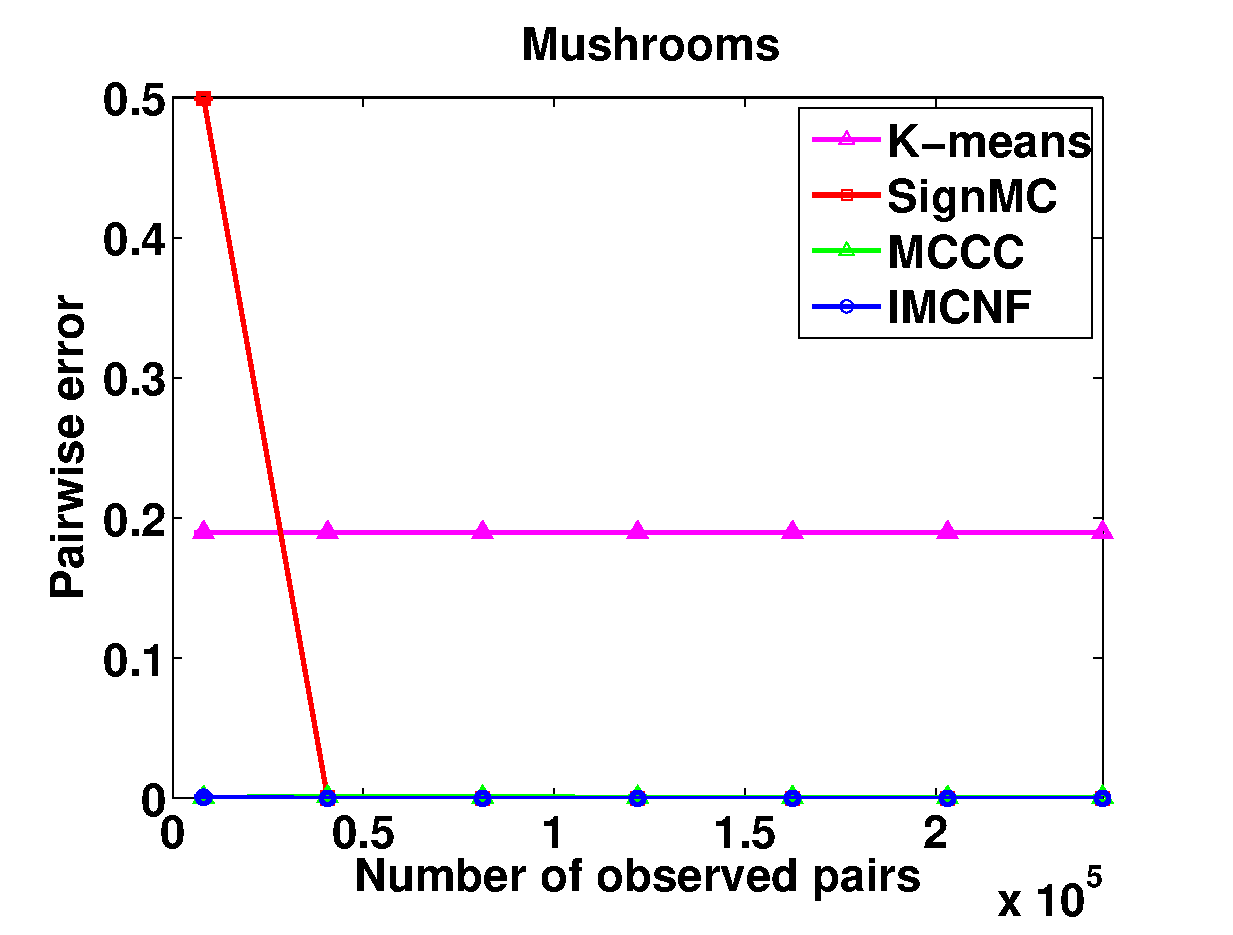
\includegraphics[width=0.32\linewidth]{figs/mushroom.eps}
    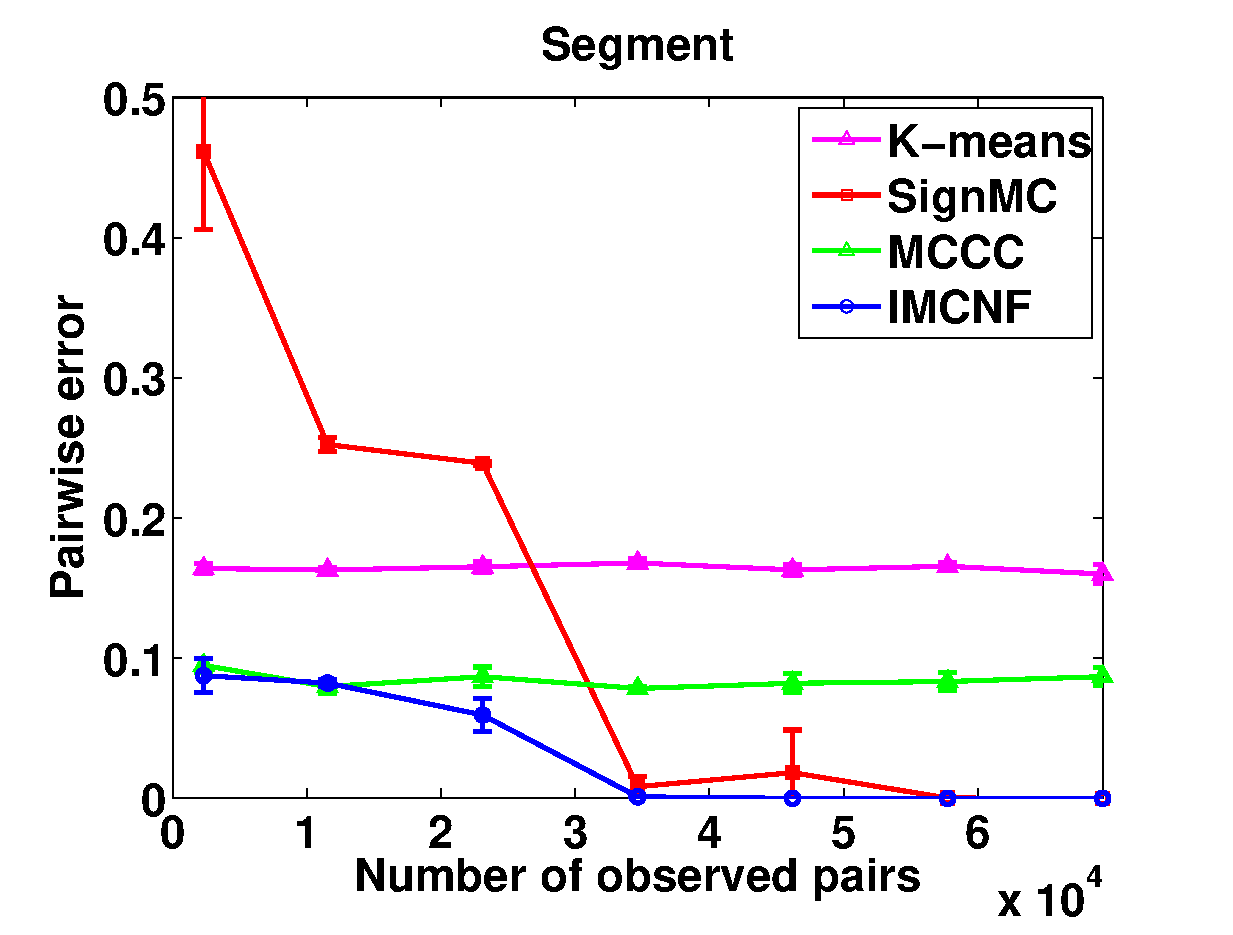
\includegraphics[width=0.32\linewidth]{figs/segment.eps}
    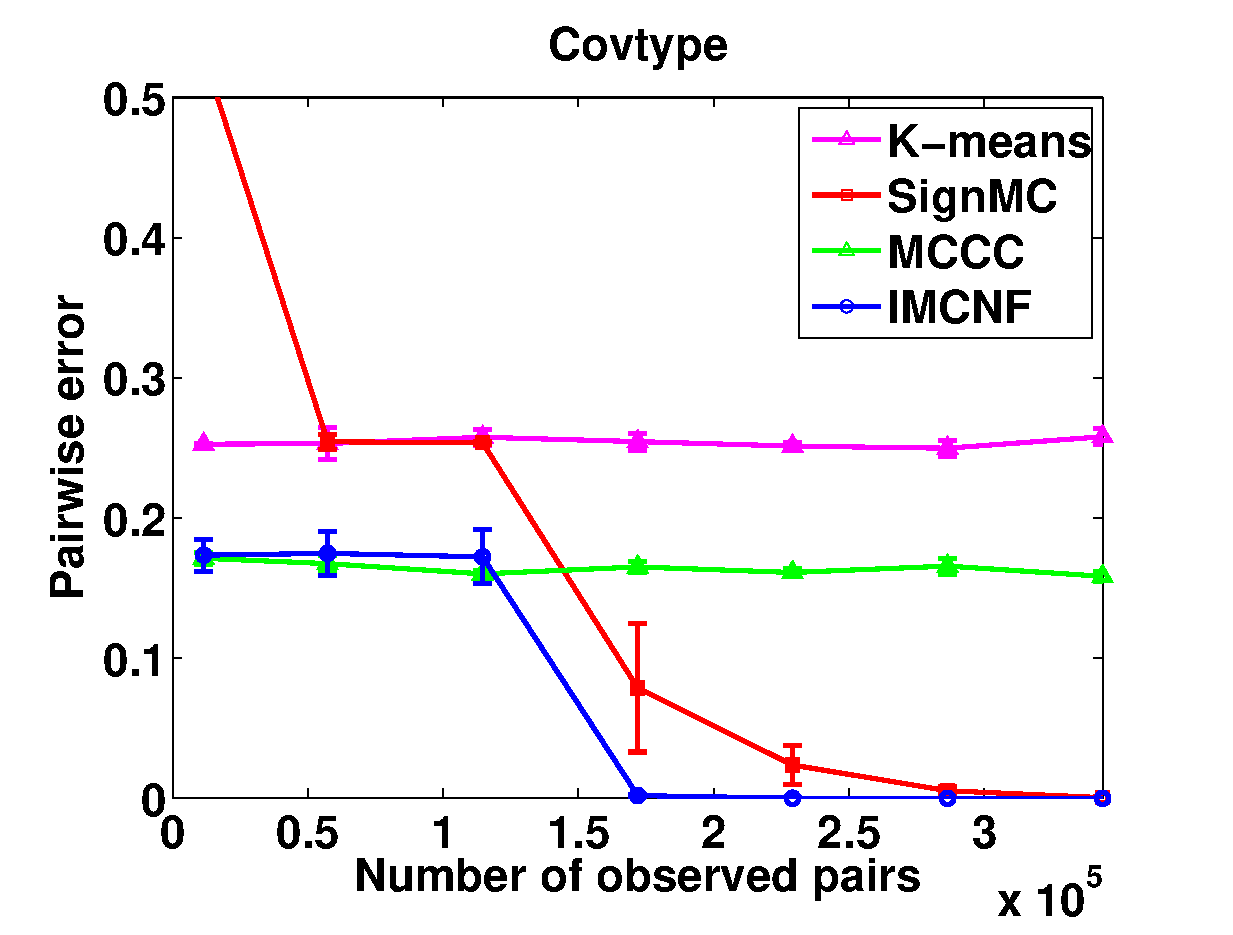
\includegraphics[width=0.32\linewidth]{figs/covtype.eps}
  \caption{Performance of various semi-supervised clustering methods on real-world data sets.  For the Mushrooms data set
  where features are perfect, both MCCC and IMCNF can output the ground-truth clustering with $0$ error rate.
  For Segment and Covtype where
  features are more noisy, IMCNF model outperforms MCCC as its error decreases given more constraints.}
  \label{fig:semi_clustering}
\end{figure}

\subsubsection{Noisy Image Classification}
\label{sec:exp.noisy_classification}
%{\bf \noindent Application: multiclass classification on noisy images.}
Finally, we consider noisy image classification problem as an application of low-rank matrix
learning with corrupted observations.
%One application of robust PCA is (sparse) noise removal for images.
In this problem, we are given a set of correlated images in which a few of pixels are corrupted,
and the task is to denoise the images so that one can classify the images correctly.
Since the underlying clean images are correlated and thus share an implicit
low-rank structure,
standard robust PCA could be used to identify sparse noise and recover the (low-rank
approximation of) clean images.
However, in certain cases, low-dimensional features of
images may also be available from other sources.
For example, suppose the set of images are human faces,
then the principal components of general human faces---known as Eigenface~\citep{MT91a}---could
be used as features, and such features could be helpful in the denoising process.

Motivated by the above realization, here we consider multiclass classification
on a set of noisy images from the MNIST data set.  The data set includes
$50,000$ training images and $10,000$ testing images, and each image is a $28\times28$
handwritten digit
represented as a $784$-dimensional vector.
We first pre-train both multiclass linear and kernel
SVM classifiers on the clean training images, %(which predict digit label from the input vector space).
%using LIBLINEAR~\citep{RF08a} and LIBSVM~\citep{CC01a}.
and perturb the testing image set to generate noisy images $R$.
Precisely, let $\realL \in \R^{784 \times 10000}$ be the set of (clean) testing images, where
each row denotes a pixel and each column denotes an image.  We then construct a sparse noise matrix
$\realS \in \R^{784 \times 10000}$ where $\rho_s$ of entries are randomly picked to be corrupted
by setting their values to be $255$.  The observed noisy images is thus given by
$R = \min(\realL + \realS, 255)$.  In the following, we show that by exploiting features of row and
column entities in this problem, we can better denoise the noisy images for classification.

\paragraph{Exploiting Eigendigit Features.}
We first exploit ``Eigendigit'' features to help denoising.  We take the training image set
to produce the Eigendigit features $X \in \R^{784 \times 300}$ using PCA and simply set
$Y = I$ as we do not consider any column features here.
We then input $R$ into PCP to derive a set of denoised images $\optL_{pcp}$ and
input $R$, $X$ and $Y$ (which is $I$) into PCPF (problem~\ref{eq:PCPF}) to derive another
set of denoised images $\optL_{pcpf} = X\optM$.
Both $\optL_{pcp}$ and $\optL_{pcpf}$ will be low rank approximations
of the clean images.
Note that although the Eigendigit features $X$ will not satisfy \eqref{eq:perfect_feature}
which is assumed in the derivation of PCPF,
%which is required to guarantee exact recovery of PCPF in theory,
we could heuristically incorporate it using PCPF in this circumstance because $X$ is still expected to
contain unbiased information of the low-rank approximation
of the clean digits.~\footnote{Rigorously speaking, the ground-truth $\realL$
is not even low-rank, but only approximately low-rank.}

To compare the quality of denoised images of PCP and PCPF, we input
$\optL_{pcp}$ and $\optL_{pcpf}$ to pre-trained SVMs for digit classification
and report the results in Table~\ref{tab:digit_classification}.
%To further justify the quality of denoised images in terms of practical metrics
%in real application, we consider the classification accuracy achieved
%by denoised images as the second metric.
%We pre-train both multiclass linear and kernel
%SVM classifiers on $50000$ clean training images
%to predict the digit from input vector space
%using LIBLINEAR~\cite{RF08a} and LIBSVM~\cite{CC01a}.
%We then use these trained classifiers to
%classify the denoised images from PCP and PCPF.  The results are reported in
%Table~\ref{tab:classification}.
%The column ``Clean'' denotes the accuracy on clean testing images (i.e. $\realL$),
%and the column ``Noisy'' denotes the accuracy on noisy images (i.e. $R$) without
%any denoising process.  The last two columns are accuracies on denoised
%images from PCP and PCPF respectively.
Both methods are somehow effective for denoising sparse noise, since accuracies achieved by
the denoised images are much closer to the clean images compared to the noisy images.
Furthermore, PCPF consistently achieves better accuracies than PCP under different
$\rho_s$, showing that incorporating Eigendigit features using PCPF is helpful on
denoising process for classification.

\begin{table}
  \centering
  \begin{tabular}{c|c|c|rr||c|c|c|rr}
    \multicolumn{5}{c}{linear SVM classifiers}&
    \multicolumn{5}{c}{kernel SVM classifiers}\\
    \hline
    $\rho_s$ & Clean & Noisy & PCP & PCPF &
    $\rho_s$ & Clean & Noisy & PCP & PCPF \\ \hline
    %0.05 & \multirow{4}{*}{91.96} & 77.93 & 86.94 & {\bf 87.51} &
    %0.05 & \multirow{4}{*}{98.33} & 66.14 & 95.17 & {\bf 95.74} \\
    0.1 & \multirow{3}{*}{91.96}& 59.63 & 86.33 & {\bf 87.88} &
    0.1 & \multirow{3}{*}{98.33}& 18.47 & 94.85 & {\bf 95.89} \\
    0.2 & & 38.16 & 85.94 & {\bf 87.48} &
    0.2 & & 10.32 & 94.55 & {\bf 95.48} \\
    0.3 & & 25.63 & 78.52 & {\bf 79.84} &
    0.3 & & 10.32 & 87.00 & {\bf 87.78} \\
  \end{tabular}
  \caption{Digit classification accuracy of PCP and PCPF with Eigendigit features.
    %under each sparsity of noise $\rho_s$.
    The column Clean shows
    the accuracy on $\realL$ and the column Noisy shows the accuracy on $R$.
    Denoised images from both PCP and PCPF achieve much higher accuracy than noisy images,
    and PCPF further outperforms PCP by incorporating Eigendigit features.}
  \label{tab:digit_classification}
\end{table}

\paragraph{Exploiting both Eigendigit and Label-relevant Features}
\begin{figure}[t]
  \centering
  %\begin{tabular}{cc}
      %\subfloat[$\rho_s = 0.05$]{
      %\includegraphics[width=0.4\linewidth]{figs/digit_rhos_005.eps}
      %\label{fig:digit_rhos_005}}
      \subfloat[Linear SVM, $\rho_s = 0.1$]{
      \includegraphics[width=0.32\linewidth]{figs/digit_rhos_01.eps}
      \label{fig:digit_rhos_01}
      }
      \subfloat[Linear SVM, $\rho_s = 0.2$]{
    \includegraphics[width=0.32\linewidth]{figs/digit_rhos_02.eps}
    \label{fig:digit_rhos_02}}
      \subfloat[Linear SVM, $\rho_s = 0.3$]{
    \includegraphics[width=0.32\linewidth]{figs/digit_rhos_03.eps}
    \label{fig:digit_rhos_03}}\\
      \subfloat[Kernel SVM, $\rho_s = 0.1$]{
      \includegraphics[width=0.32\linewidth]{figs/svm_digit_rhos_01.eps}
      \label{fig:svm_digit_rhos_01}
      }
      \subfloat[Kernel SVM, $\rho_s = 0.2$]{
    \includegraphics[width=0.32\linewidth]{figs/svm_digit_rhos_02.eps}
    \label{fig:svm_digit_rhos_02}}
      \subfloat[Kernel SVM, $\rho_s = 0.3$]{
    \includegraphics[width=0.32\linewidth]{figs/svm_digit_rhos_03.eps}
    \label{fig:svm_digit_rhos_03}}
  %\end{tabular}
    \caption{Digit classification accuracy of various methods with both Eigendigit and label-relevant features.
    For each $\rho_s$, we construct the label-relevant features $Y$ with different quality by varying $\rho_f$.
    The results show that PCPNF-w/Y is able to better exploit noisy label-relevant features $Y$.}
  \label{fig:digit_exp_pcpgf}
\end{figure}
In addition to the Eigendigit features $X$, now we further exploit features for column entities.
Ideally, the column features $Y$ may describe the relevant information between images, which could be
extremely useful for classification.  Thus, we generate the ``label-relevant'' features $Y$ for column entities
as follows.
Let $Y^* \in \R^{10000\times 10}$ be a perfect column feature matrix where the
$i$-th column of $Y^*$ is the indicator vector of digit $i-1$ (so $Y^*$ contains
ground-truth label information).
%~\footnote{Rigorously speaking, $Y^*$ ``almost'' contains all ground-truth label information
%since it tells us which images are in the same class, but does not tell us which
%class (digit) they belongs to.}).
We then randomly pick $\rho_f$ of rows in $Y^*$ and shuffle
these rows to form $\tilde{Y}$, which correspondingly means that $10,000\times\rho_f$ images
have noisy relevant information in $\tilde{Y}$.  Finally, we form the column feature
$Y \in \R^{10000\times 50}$ which spans $\tilde{Y}$.  Thus, the quality of $Y$ depends on the parameter
$\rho_f \in [0, 1]$ and smaller $\rho_f$ results in better label-relevant features.

We consider four approaches for denoising in the following experiment.
The first two baseline methods are PCP and PCPF with
only Eigendigit features $X$.
%, denoted by PCP and PCPF respectively.
Both methods are the ones we considered in the previous experiment
which do not take label-relevant features into account.
Moreover, we consider using PCPF and PCPNF to incorporate
{\it both} the Eigendigit features $X$ and the label-relevant features $Y$ for denoising,
and we name them as ``PCPF-w/Y'' and ``PCPNF-w/Y''
to emphasize that they embed the label-relevant features $Y$.
We apply each method to denoise noisy images under different $\rho_f$ and $\rho_s$
and examine the quality of denoised images
by testing the accuracies they achieve in pre-trained SVMs.

The results are shown in Figure~\ref{fig:digit_exp_pcpgf}.
In each figure, we fix the sparsity of noise
$\rho_s$ and try to recover the clean images using each method with different quality of $Y$.
We can see that the perfect label-relevant features are extremely useful, as
when $\rho_f = 0$, recovered images from both PCPF-w/Y and PCPNF-w/Y
achieve even much higher accuracies compared to the clean images
(reported in Table~\ref{tab:digit_classification}).  However, once $\rho_f$ increases,
PCPF-w/Y quickly fails as its accuracy drops drastically (accuracies
become much lower than $70$ for $\rho_f > 0.5$ and thus are not shown in figures).
%This phenomenon is again because the information in $Y$ becomes partially misleading,
%and PCPF-w/Y is sensitive to such noisy $Y$ and is severely trapped by noisy features.
On the other hand, we see that PCPNF-w/Y performs
much better than PCPF-w/Y on exploiting noisy label-relevant features, as
it still achieves better accuracies compared to both PCPF and PCP when $\rho_f > 0$.
The results again demonstrate
the effectiveness of our proposed model on exploiting noisy side information.

\begin{comment}
\begin{table}
  \centering
  \begin{tabular}{l|r||r|r|r|r}
  $\rho_s$ & $\rho_f$ of $Y$ & PCP & PCPF & PCPF-w/Y & PCPNF-w/Y \\
  \hline
      \multirow{5}{*}{0.05} & 0.0 & 86.94 & 87.51 & 99.93 & {\bf 99.94} \\
                            & 0.2 & 86.94 & 87.51 & 82.09 & {\bf 91.65} \\
                            & 0.5 & 86.94 & 87.51 & 46.39 & {\bf 90.73} \\
                            & 0.8 & 86.94 & 87.51 & 9.95 & {\bf 90.56} \\
                            & 1.0 & 86.94 & 87.51 & 9.74 & {\bf 90.55} \\
      \hline
      \multirow{5}{*}{0.1} & 0.0 & 86.33 & 87.88 & 99.92 & {\bf 99.93} \\
                            & 0.2 & 86.33 & 87.88 & 81.72 & {\bf 91.72} \\
                            & 0.5 & 86.33 & 87.88 & 40.50 & {\bf 90.66} \\
                            & 0.8 & 86.33 & 87.88 & 9.90 & {\bf 90.32} \\
                            & 1.0 & 86.33 & 87.88 & 9.74 & {\bf 90.32} \\
      \hline
      \multirow{5}{*}{0.2} & 0.0 & 85.94 & 87.48 & {\bf 99.94} & 99.93 \\
                            & 0.2 & 85.94 & 87.48 & 74.70 & {\bf 89.68} \\
                            & 0.5 & 85.94 & {\bf 87.48} & 29.59 & {86.22} \\
                            & 0.8 & 85.94 & {\bf 87.48} & 9.75 & {85.55} \\
                            & 1.0 & 85.94 & {\bf 87.48} & 9.74 & {85.49} \\
      \hline
      \multirow{5}{*}{0.3} & 0.0 & 78.52 & 79.84 & {\bf 99.94} & 94.03 \\
                           & 0.2 & 78.52 & 79.84 & 74.75 & {\bf 85.54} \\
                           & 0.5 & 78.52 & 79.84 & 14.84 & {\bf 80.45} \\
                           & 0.8 & 78.52 & {\bf 79.84} & 9.74 & 79.34 \\
                           & 1.0 & 78.52 & {\bf 79.84} & 9.74 & 79.25 \\

      %\multirow{4}{*}{91.96} & 77.93 & 86.94 & {\bf 87.51}\\
      %   0.1 & & 59.63 & 86.33 & {\bf 87.88} \\
      %   0.2 & & 38.16 & 85.94 & {\bf 87.48} \\
      %   0.3 & & 25.63 & 78.52 & {\bf 79.84} \\
  \end{tabular}
\end{table}
\end{comment}

\section{Related Work}
\label{sec:related}
Learning a low-rank matrix from imperfect observations is an expansive domain in machine learning
including many fundamental problems, such as Principal
Component Analysis (PCA)~\citep{Harold33a}, matrix completion~\citep{Candes09a}, low-rank matrix
sensing~\citep{Zhong15a} and robust PCA~\citep{Wright09a}.  While each of the above topics
is an independent research area burgeoning in recent years, our main focus is to
study the usefulness of side information in low-rank matrix learning where
the observations are partial and/or corrupted in both theoretical and practical
aspects.

% One important instance of low-rank matrix learning is matrix completion problem, where
% the goal is to learn the underlying low-rank matrix given only partial entries are observed.
Learning a low-rank matrix from partial observations is well-known as
matrix completion problem, which has been successfully applied
to many machine learning tasks including recommender systems~\citep{Koren09a},
social network analysis~\citep{Hsieh12a, Chiang14a} and clustering~\citep{Chen14a}.
Several theoretical foundations have also been established.
One of the most striking results is the exact recovery guarantee provided by
\citet{Candes09a} and \citet{Candes12a}
where the authors showed that $O(n\polylog{n})$ observations are sufficient
for exact recovery with high probability,
provided that entries are uniformly sampled at random.  Several works also study
recovery under non-uniform distributional assumptions~\citep{SN12a},
distribution-free settings~\citep{Shamir14a} and noisy observations~\citep{RK10a, EC10b}.

A few research papers also consider side information in the matrix completion setting
\citep{Menon11a, Chen12a, Natarajan14a, Shin15a}.
Although most of them found that features are helpful
in certain applications~\citep{Menon11a, Shin15a}
and in the cold-start setting~\citep{Natarajan14a},
they mainly focus on the non-convex matrix factorization formulation
without any theoretical analysis on the effect of side information.
More recently, \citet{Jain13a} studied Inductive Matrix Completion (IMC) objective
to incorporate side information, and several follow-up works also
consider IMC with trace norm regularization~\citep{Xu13a, Zhong15a}.
All of them showed that recovery can be achieved by IMC with much lower sample complexity
provided perfect features.
%(which will be introduced in Section~\ref{subsec:mc.imc}).
However, as we have discussed in the paper, given imperfect features, IMC cannot recover the underlying matrix and
may even suffer from poor performance in practice.  This observation leads us to further
develop an improved model which better exploits noisy side information in learning
(see Section~\ref{subsec:propose}).

%Our proposed model is also related to the family of dirty statistical models~\cite{EY13a},
%where the model parameter is expressed as the sum of a number of parameter components,
%each of which has its own structure. Dirty statistical models have been proposed
%mostly for robust matrix completion, graphical model estimation,
%and robust PCA problem to decompose the sparse component (noise) and low-rank component (model
%parameters)~\cite{Candes11a,VC12a,AJ10a}.
%Our proposed DirtyIMC algorithm is completely different from them. We aim to decompose
%the model into two parts: the part that can be described by side information and the part
%that has to be recovered purely by observations.

Robust PCA is another prominent instance of low-rank matrix learning
from imperfect observations,
where the goal is to recover a low-rank matrix
from a full matrix in which a few of entries are arbitrarily corrupted by sparse noise.
This sparse structure of noise is common in many applications such as
image processing and bioinformatics~\citep{Wright09a}.
Researchers have also investigated several approaches to robust PCA with
theoretical guarantees~\citep{VC11a, Candes11a}.
Perhaps the most remarkable milestone is the strong guarantee
provided by~\citet{Candes11a}, in which the authors showed that under mild conditions,
low-rank and sparse structure are exactly distinguishable.
Several extensions of robust PCA
have also been considered, such as robust PCA with column-sparse errors~\citep{Xu10a},
with missing data~\citep{Candes11a, Chen13a} and with compressed data~\citep{Ha15a}.

However, unlike matrix completion, there is little research that directly exploits
side information in the robust PCA problem, leaving the advantage of side information
in robust PCA unexplored.
Though it may appear that one can extend the analysis of side information in matrix completion
to robust PCA as both problems share certain similarities,
%it may appear a positive sign to exploit side information in robust PCA.
%However, %as we will discuss in Section~\ref{subsec:robust.pcpf},
the robust PCA problem
is still essentially different---in fact harder---from matrix completion in many aspects.
In particular, matrix completion has been mostly used for {\it missing value estimation},
where the emphasis is to accurately recover the missing entries given trustable, partial
observations, while robust PCA is a {\it matrix separation problem} where
one has to identify the corrupted entries given full yet untrustable observations.
%In particular, in matrix completion, locations of missing entries are already known,
%while in robust PCA the support of corrupted entries is unknown.
This difference naturally precludes a direct extension from the analyses of
matrix completion to robust PCA.  Nevertheless, \citet{Chiang16a}
has recently shown that given perfect features, exact recovery of higher-rank matrices becomes
attainable in the robust PCA problem, indicating that side information in robust PCA
can be exploited.
In this paper, we extend~\citet{Chiang16a} and develop a more general model which can
further exploit noisy side information to help solve the robust PCA problem.

Another model that shares certain similarities to robust PCA with side information is
Low-Rank Representation (LRR), which emerged from the subspace clustering problem~\citep{Liu10a, Liu13a}.
Given that the observed data matrix is corrupted by sparse errors,
LRR model assumes that the underlying low-rank matrix can be represented by a linear
combination of a provided dictionary.
Interestingly, LRR can be thought of as a special
case of the proposed PCPF model (see Section~\ref{subsec:propose})
where the given dictionary serves as
the row features $X$.  Our problem setting is also more general than LRR as we
consider incorporating both row and column features to help recovery.

\section{Conclusions}
\label{sec:conclusion}
In this paper, we study the effectiveness of side information for
low-rank matrix learning from missing and corrupted observations.
We propose a general model (problem~\eqref{eq:general_form}) which incorporates both perfect and noisy side information
by balancing information from features and observations simultaneously,
from which we can derive several instances of the model, including IMCNF and PCPNF,
that better solve matrix completion and robust PCA by leveraging side information.
In addition, we provide a formal analysis to justify the effectiveness of side information
in the proposed model, in which we quantify the quality of features and show that
the sample complexity of learning can be asymptotically improved given sufficiently informative
features, provided a small enough noise level.
This analysis therefore quantifies the merits of side information in our model for low-rank matrix learning in theory.
Finally, we verify our model in several synthetic experiments
as well as in real-world machine learning applications including
relationship prediction, semi-supervised clustering and noisy image classification.
By viewing each application as a low-rank matrix learning problem from missing or corrupted observations
given certain additional features,
we show that employing our model results in competitive
algorithms whose performance is comparable to or better than other state-of-the-art approaches.
All of our results consistently demonstrate that the proposed model learns
the low-rank matrix from missing and corrupted observations more effectively
by properly exploiting side information.


% Acknowledgements should go at the end, before appendices and references

\acks{We would like to acknowledge support for this research
from CCF-1320746, IIS-1546452 and CCF-1564000.}

% Manual newpage inserted to improve layout of sample file - not
% needed in general before appendices/bibliography.

% Note: in this sample, the section number is hard-coded in. Following
% proper LaTeX conventions, it should properly be coded as a reference:
\appendix
\section{Proofs}
\subsection*{Preliminary Lemmas}
We first introduce two lemmas required in the proof of Lemma~\ref{lemma:rad_bound1}.
These two lemmas provide bounds on the Rademacher complexity of the function
class with bounded trace norm and $\ell1$ norm respectively.
%which will be used for proving Lemma~\ref{lemma:rad_bound0}.
%where the class of linear functions are constrained by a bounded trace norm.
\begin{lemma}
  \label{lemma:rad_bound_nuclear}
  Let $S_w = \{W \in \R^{n\times n}\mid \|W\|_* \leq \wmax\}$ and
  $\amax = \max_i \|A_i\|_2$, where each $A_i \in \R^{n\times n}$,
  then:
  \begin{equation*}
    \Ex{\sigma}{\sup_{W\in S_w}\frac{1}{m} \sum_{i=1}^m \sigma_i \trace{WA_i}}
    \leq 2\amax\wmax\sqrt{\frac{\log{2n}}{m}}.
  \end{equation*}
\end{lemma}
\begin{proof}
  This Lemma is directly from the Lemma 3 in~\citet{Hsieh15a}.
\end{proof}
%\begin{proof}
%This Lemma is a special case of Theorem 1 in~\citet{SK08a} with the fact that the
%dual norm of the matrix 2-norm is trace norm.
%\end{proof}

\begin{lemma}
  \label{lemma:rad_bound_sparse}
  Let $S_w = \{W \in \R^{n_1\times n_2}\mid \|W\|_1 \leq \wmax\}$, and each $E_i$
  is in the form of $E_i = \be_x \be_y^T$,
  where $\be_x \in \R^{n_2}$, $\be_y \in \R^{n_1}$ are two unit vectors.  Then:
  \begin{equation*}
    \Ex{\sigma}{\sup_{W \in S_w} \frac{1}{m}\sum_{i=1}^m
    \sigma_{i}\trace{W E_i}}
    \leq \wmax \sqrt{\frac{2\log{(2n_1n_2)}}{m}}.
  \end{equation*}
\end{lemma}
\begin{proof}
This Lemma is a special case of Theorem 1 in~\citet{SK08a} with the fact that
$\|E_i\|_\infty := \max_{a,b}|(E_i)_{ab}|= 1$.
\end{proof}

\subsection*{Proof of Lemma~\ref{lemma:rad_bound1}}
\begin{proof}
First, we can use a standard Rademacher contraction principle (e.g. Lemma~5 in~\citealp{RM03a})
to bound
$\rad(F_\Theta)$ to be:
\begin{align*}
  \rad(F_{\Theta}) \leq&
L_\ell \Ex{\sigma}{\sup_{\theta\in\Theta} \frac{1}{m} \sum_{\sigma=1}^m
  \sigma_{\alpha}(XMY^T+N+S)_{i_\alpha j_\alpha}} \nonumber \\
    %&= L_\ell \Ex{\sigma}{\sup_{\|M\|_*\leq\mmax} \frac{1}{m}\sum_{\sigma=1}^m
    %    \sigma_{\alpha}\bx_{i_\alpha}^TM\by_{j_\alpha}}
    %+L_\ell \Ex{\sigma}{\sup_{\|N\|_*\leq\nmax} \frac{1}{m}\sum_{\sigma=1}^m
    %  \sigma_{\alpha}N_{i_\alpha j_\alpha}} \\
    =&
    L_\ell \Ex{\sigma}{\sup_{\|M\|_*\leq\mmax} \frac{1}{m}\sum_{\alpha=1}^m
              \sigma_{\alpha}\trace{M\by_{j_\alpha}\bx_{i_\alpha}^T}}
    + L_\ell\Ex{\sigma}{\sup_{\|N\|_*\leq\nmax} \frac{1}{m}\sum_{\alpha=1}^m
      \sigma_{\alpha}\trace{N\be_{j_\alpha}\be_{i_\alpha}^T}}\\
    &+ L_\ell\Ex{\sigma}{\sup_{\|S\|_1\leq\smax} \frac{1}{m}\sum_{\alpha=1}^m
      \sigma_{\alpha}\trace{S\be_{j_\alpha}\be_{i_\alpha}^T}}\\
    \leq&
    %2L_\ell\bigg(\mmax\max_{i,j}\|\by_j\bx_i^T\|_2
    %+ \nmax \bigg) \sqrt{\frac{\log{2n}}{m}},
    2L_\ell\mmax\max_{i,j}\|\by_j\bx_i^T\|_2 \sqrt{\frac{\log{2d}}{m}}
    + 2L_\ell\nmax \sqrt{\frac{\log{2n}}{m}} + L_\ell\smax \sqrt{\frac{2\log{(2n_1n_2)}}{m}}
    \end{align*}
    where the last inequality is derived by applying Lemma~\ref{lemma:rad_bound_nuclear} and Lemma~\ref{lemma:rad_bound_sparse}.
    Moreover, since $\max_{i,j} \|\by_j\bx_i^T\|_2 = \max_j \|\by_j\|_2
    \max_i\|\bx_i\|_2$, we can thus upper bound $\rad(F_{\Theta})$ by:
    \begin{equation}
    %  \Ex{\Omega}{\rad(F_\Theta)} \leq 2L_\ell \bigg( \mmax \xmax \ymax +
    %\nmax \bigg) \sqrt{\frac{\log{2n}}{m}}.
      {\rad(F_{\Theta})} \leq 2L_\ell \mmax \xmax \ymax \sqrt{\frac{\log{2d}}{m}}
    +2L_\ell\nmax \sqrt{\frac{\log{2n}}{m}}
    +L_\ell\smax \sqrt{\frac{2\log{(2n_1n_2)}}{m}}.
    \label{eq:first_rad_bound}
    \end{equation}

However, in some circumstances, the above bound~\eqref{eq:first_rad_bound}
is too loose for sample complexity analysis.
%However, directly using the above bound to the function class $F_\Theta$ will lead a undesired loose bound.
%As a result, we need to be more carefully to bound the model complexity.
To deal with these cases, we follow \citet{Shamir14a} to derive a tighter bound on the trace norm of residual (i.e. $\nmax$).
%we need to deal with these cases with a tighter bound
%on trace norm of residual (i.e. $\nmax$).  The following bound mostly follows the proof steps
%in~\citet{Shamir14a},
%which provides a tighter bound
%on trace-norm regularized function class.
To begin with, we rewrite $\rad(F_{\Theta})$ as:
\begin{align*}
  \rad(F_{\Theta}) = \Ex{\sigma}{\sup_{f\in F_{\Theta}}\frac{1}{m} \sum_{\alpha=1}^m \sigma_\alpha \ell(f(i_\alpha, j_\alpha), R_{i_\alpha, j_\alpha}))}
  = \Ex{\sigma}{\sup_{f\in F_{\Theta}}\frac{1}{m} \sum_{(i,j)}\Gamma_{ij} \ell(f(i,j), R_{ij})},
\end{align*}
where $\Gamma \in \R^{n_1 \times n_2}$, $\Gamma_{ij} = \sum_{\alpha:i_\alpha = i, j_\alpha = j} \sigma_\alpha$.
Now, using the same trick in~\citet{Shamir14a}, we can divide $\Gamma$ based on the ``hit-time'' of each $(i, j) \in \Obs$, with
some threshold $p > 0$ whose value will be set later.  Formally, let $h_{ij} = |\{\alpha: i_\alpha = i, j_\alpha = j\}|$,
and let $A, B\in \R^{n_1 \times n_2}$ be defined by:
\begin{equation*}
  A_{ij} = \begin{cases}
    \Gamma_{ij}, &\text{ if $h_{ij} > p$}, \\
    0, &\text{ otherwise}.
    \end{cases}
  \hspace{1cm}
  B_{ij} = \begin{cases}
    0, &\text{ if $h_{ij} > p$}, \\
    \Gamma_{ij}, &\text{ otherwise}.
  \end{cases}
\end{equation*}
By construction, $\Gamma = A+B$.  Therefore, we can separate $\rad(F_{\Theta})$ to be:
\begin{equation}
  \rad(F_{\Theta}) = \Ex{\sigma}{\sup_{f\in F_{\Theta}}\frac{1}{m} \sum_{(i,j)}A_{ij} \ell(f(i,j), R_{ij})}
  +\Ex{\sigma}{\sup_{f\in F_{\Theta}}\frac{1}{m} \sum_{(i,j)}B_{ij} \ell(f(i,j), R_{ij})}.
  \label{eq:separate_by_hit}
\end{equation}
For the first term in \eqref{eq:separate_by_hit},
since $|\ell(f(i,j), R_{ij})| \leq \bmax$, it can be upper bounded by:
\begin{equation*}
  \Ex{\sigma}{\sup_{f\in F_{\Theta}}\frac{1}{m} \sum_{(i,j)}A_{ij} \ell(f(i,j), R_{ij})} \leq
  \frac{\bmax}{m} \Ex{\sigma}{\sum_{(i,j)}|A_{ij}|} \leq \frac{\bmax}{\sqrt{p}}
\end{equation*}
where the last inequality is derived by applying Lemma~10 in \citet{Shamir14a}.
Now consider the second term of~\eqref{eq:separate_by_hit}.
Again, by Rademacher contraction principle,
it can be upper bounded by:
\begin{align}
  &\frac{L_\ell}{m} \Ex{\sigma}{\sup_{f \in F_{\Theta}}\sum_{(i,j)}B_{ij} f(i,j)}\nonumber\\
  = &\frac{L_\ell}{m}\Ex{\sigma}{\sup_{\|M\|_*\leq\mmax} \sum_{(i,j)} B_{ij}\bx_i^TM\by_j}
    + \frac{L_\ell}{m}\Ex{\sigma}{\sup_{\|N\|_*\leq\nmax}\sum_{(i,j)} B_{ij}N_{ij}}
    + \frac{L_\ell}{m}\Ex{\sigma}{\sup_{\|S\|_1\leq\smax}\sum_{(i,j)} B_{ij}S_{ij}}.
    \label{eq:lower_hit}
\end{align}
We can again upper bound the first and third term of~\eqref{eq:lower_hit}
using Lemma~\ref{lemma:rad_bound_nuclear} and Lemma~\ref{lemma:rad_bound_sparse}.  Precisely, the first term can be upper bounded by:
\begin{align*}
      \frac{L_\ell}{m} \Ex{\sigma}{\sup_{\|M\|_*\leq\mmax}\sum_{\alpha=1}^m
       \sigma_\alpha \bx_{i_\alpha}^TM\by_{j_\alpha}}
       = L_\ell \Ex{\sigma}{\sup_{\|M\|_*\leq\mmax} \frac{1}{m}\sum_{\alpha=1}^m
     \sigma_\alpha\trace{M\by_{j_\alpha}\bx_{i_\alpha}^T}}
     %&\leq 2L_\ell\mmax\max_{i,j}\|\by_j\bx_i^T\|_2 \sqrt{\frac{\log{2d}}{m}} \\
     \leq 2L_\ell\mmax\xmax\ymax\sqrt{\frac{\log{2d}}{m}},
\end{align*}
and the third term of \eqref{eq:lower_hit} is upper bounded by:
\begin{equation*}
    L_\ell\Ex{\sigma}{\sup_{\|S\|_1\leq\smax} \frac{1}{m}\sum_{\alpha=1}^m
      \sigma_{\alpha}\trace{S\be_{j_\alpha}\be_{i_\alpha}^T}}\\
    \leq L_\ell\smax \sqrt{\frac{2\log{(2n_1n_2)}}{m}}.
\end{equation*}
In addition, by applying H{\"o}lder's inequality, the second term of~\eqref{eq:lower_hit} is upper bounded by:
\begin{align*}
  \frac{L_\ell}{m}\Ex{\sigma}{\sup_{\|N\|_*\leq\nmax}\sum_{(i,j)} B_{ij}N_{ij}}
  \leq
  \frac{L_\ell}{m} \sup_{N:\|N\|_*\leq\nmax} \|B\|_2 \|N\|_* = \frac{L_\ell\nmax}{m} \Ex{\sigma}{\|B\|_2}
  \leq \frac{2.2CL_\ell \nmax \sqrt{p}(\sqrt{n_1} + \sqrt{n_2})}{m},
\end{align*}
where the last inequality is derived by applying Lemma~11 in \citet{Shamir14a}.  %Furthermore
%where the second last inequality is again derived by Lemma~\ref{lemma:rad_bound_nuclear}.
%and the last
%inequality is because $\max_{i,j} \|\by_j\bx_i^T\|_2 = \max_j \|\by_j\|_2\max_i\|\bx_i\|_2$.  Therefore, by
Therefore, putting all of the above upper bounds to~\eqref{eq:separate_by_hit} and choosing $p$ to be
$m\bmax/(2.2CL_\ell\nmax(\sqrt{n_1}+\sqrt{n_2}))$, we obtain another upper bound on
$\rad(F_{\Theta})$ as:
\begin{equation}
  {\rad(F_{\Theta})} \leq 2L_\ell\mmax \xmax \ymax \sqrt{\frac{\log{2d}}{m}} + \sqrt{9CL_\ell\bmax\frac{\nmax(\sqrt{n_1}+\sqrt{n_2})}{m}}
    %\Ex{\Omega}{\rad(F_\Theta)} \leq 2L_\ell\mmax \xmax \ymax \sqrt{\frac{\log{2n}}{m}} + \sqrt{9CL_\ell\bmax\frac{\nmax(\sqrt{n_1}+\sqrt{n_2})}{m}}.
  +L_\ell\smax \sqrt{\frac{2\log{(2n_1n_2)}}{m}}.
    \label{eq:second_rad_bound}
\end{equation}
Lemma~\ref{lemma:rad_bound1} thus follows by combining \eqref{eq:first_rad_bound} and \eqref{eq:second_rad_bound}.
\end{proof}

\subsection*{Proof of Lemma~\ref{lemma:trM_bound}}
\begin{proof}
To begin with, we have:
  \begin{equation*}
    \|X_\mu^T\realL Y_\nu\|_2 \leq \|X_\mu\|_2\|\realL\|_2\|Y_\nu\|_2 \leq
    \sigma_x\sigma_y\|\realL\|_*,
  \end{equation*}
  where $\sigma_x$ (or $\sigma_y$) is the largest singular value of $X_\mu$ (or $Y_\nu$).
  Therefore, by the definition of $\wM$, we have:
  \begin{align}
    \|\wM\|_*
    \leq d \|\wM\|_2
    = d\|(X_{\mu}^TX_\mu)^{\dagger}X_\mu^T\realL Y_\nu(Y_\nu^TY_\nu)^{\dagger}\|_2
    \leq \frac{\sigma_x\sigma_yd\|\realL\|_*}{\sigma_{xm}^2\sigma_{ym}^2},
    \label{eq:trM_bound_tmp}
  \end{align}
  where $\sigma_{xm}$ (or $\sigma_{ym}$)
  is the smallest non-zero singular value of $X_\mu$ (or $Y_\nu$).
  Furthermore, by the construction of
  $X_\mu$ and $Y_\nu$, we have $\sigma_{xm} \geq \mu\sigma_x$ and $\sigma_{ym} \geq \nu\sigma_y$.
  We can further lower bound $\sigma_x$ (and $\sigma_y$) by:
  \begin{equation*}
    \sigma_x^2 = \|X_\mu\|_2^2 = \|X\|_2^2 \geq \frac{\|X\|^2_F}{d} \geq \frac{n\min\|\bx_i\|^2}{d}
    \geq \frac{n\gamma^2\xmax^2}{d}.
  \end{equation*}
  %Now, using Lemma~\ref{lemma:singular_value_bound}, we have:
  Therefore, from \eqref{eq:trM_bound_tmp}, we can further bound $\|\wM\|_*$ by:
  \begin{align*}
    \|\wM\|_*  \leq \frac{d\|\realL\|_*}{\mu^2\nu^2\sigma_x\sigma_y}
    %&\leq \frac{\|R\|_*\hat{d}}{C'\gamma^2\mu^2\nu^2\xmax\ymax} \\
    %\leq \frac{\|\realL\|_*\hat{d}}{C'\sqrt{n_1 n_2}\gamma^2\mu^2\nu^2\xmax\ymax},
    \leq \frac{d^2\|\realL\|_*}{\mu^2\nu^2\gamma^2\xmax\ymax\sqrt{n_1 n_2}}.
  \end{align*}
  The lemma is thus concluded by the fact that
  $\|\realL\|_* \leq C_L \sqrt{n_1 n_2}$.
\end{proof}

\subsection*{Proof of Theorem~\ref{thm:gen_bound}}
\begin{proof}
  The claim is directly proved by plugging Lemma~\ref{lemma:rad_bound1} - \ref{lemma:trM_bound}
  to Lemma \ref{lemma:expect_l_risk_2}, in which $\hat{R}_\ell(f^*) = 0$ because
  $(\hat{M}, \realL-X \hat{M} Y^T, \realS) \in \Theta$ and such an instance makes
  $\hat{R}_\ell = 0$.
\end{proof}

\subsection*{Proof of Theorem~\ref{thm:sample_comp_mc}}
\begin{proof}
  Note that since $\realS = \optS = 0$ in matrix completion case, we have:
  \begin{equation*}
    R_\ell(f^*) = \Ex{(i,j)\sim\dist}{\ell(X\optM Y^T_{ij}, \be_i^T\realL\be_j)}.
  \end{equation*}
  The claim therefore directly follows from Theorem~\ref{thm:gen_bound}
  by setting $R_\ell(f^*) < \epsilon$.
\end{proof}

\subsection*{Proof of Theorem~\ref{thm:example0}}
\begin{proof}
  By the construction of $X$ and $Y$, we can rewrite them as follows:
  \begin{align}
    X = \sum_{i=1}^{t-1}\bu_i\be_i^T + \sum_{i=t}^d\tilde{\bu}_i\be_i^T, \hspace{1cm}
    Y = \sum_{i=1}^{t-1}\bv_i\be_i^T + \sum_{i=t}^d\tilde{\bv}_i\be_i^T,
    \label{eq:example0_feature}
  \end{align}
  where for each $\tilde{\bu}_i$, $\tilde{\bu}_i^T\bu_j = 0,  \forall j$.  Therefore, we can upper
  bound $\nmax$ by:
  \begin{align*}
    \|\realL-X\hat{M}Y^T\|_* &= \|\tilde{U}\tilde{U}^T\realL + \realL\tilde{V}\tilde{V}^T - \tilde{U}\tilde{U}^T\realL\tilde{V}\tilde{V}^T\|_* \\
      &\leq 2\|\tilde{U}\tilde{U}^TU\Sigma V^T\|_* + \|U\Sigma V^T\tilde{V}\tilde{V}^T\|_* \\
      &\leq 3\sum_{i=t}^k \sigma_i,
  \end{align*}
  where $\tilde{U}$, $\tilde{V}$ are the second term of $X$ and $Y$ in \eqref{eq:example0_feature}.
  Moreover, we have $\sigma_i = o(\sqrt{n})$ for all $i \geq t$.
  To see this,
  suppose $\sigma_p = \Omega(\sqrt{n})$ for any $t \leq p \leq k $, then:
  \begin{equation*}
    \lim_{n\rightarrow\infty}\frac{\sigma_t}{\sqrt{n}} \geq
    \lim_{n\rightarrow \infty}\frac{\sigma_p}{\sqrt{n}} > 0,
  \end{equation*}
  leading a contradiction to the definition of $\sigma_t$.
  Therefore we can conclude:
  \begin{equation*}
    \nmax = \|\realL-X\hat{M}Y^T\|_* \leq 3\sum_{i=t}^k \sigma_i \leq 3k \times o(\sqrt{n}) = o(\sqrt{n}),
  \end{equation*}
  and the Theorem is thus proved by plugging the above bound on $\nmax$ to Theorem~\ref{thm:sample_comp_mc}.
\end{proof}

\subsection*{Proof of Theorem~\ref{thm:sample_comp_gen}}
\begin{proof}
  The sample complexity claim directly follows from Theorem~\ref{thm:gen_bound} by setting $R_\ell(f^*) < \epsilon$,
  and the claim of $\proj{\Obs^\perp}(\optS) = 0$ is directly from the construction of
  Algorithm~\ref{alg:general_form} as discussed in Section~\ref{subsec:optimization}.
\end{proof}

\vskip 0.2in
\bibliography{17-112}


\end{document}
